% !BIB program = biber

\documentclass[doc]{apa6}
\usepackage{longtable}
\usepackage[american]{babel}
\usepackage{endnotes}
\let\footnote=\endnote
\usepackage[bitstream-charter]{mathdesign}
\usepackage{csquotes}
\usepackage{booktabs}
\usepackage[style=apa,sortcites=true,sorting=nyt,backend=biber]{biblatex}
\usepackage{amsmath}
\usepackage{subfigure}
\usepackage{placeins}
\DeclareLanguageMapping{american}{american-apa}
\addbibresource{simon11.bib}
\newcommand{\cat}[1]{\sc{#1}}
\newcommand{\abs}[1]{\lvert#1\rvert}
\newcommand{\stimulus}[1]{\textsc{#1}}


% ---------- watermark -----------
\usepackage[firstpage]{draftwatermark}
\SetWatermarkAngle{0}
\SetWatermarkFontSize{0.25cm}
\SetWatermarkVerCenter{1.25cm}
\SetWatermarkLightness{0.5}
\SetWatermarkHorCenter{14cm}
\SetWatermarkText{\shortstack[l]{
De Deyne, S., Navarro D. J., Perfors, A. and Storms, G. (2016). Structure at \\
every scale: A semantic network account of the similarities between very \\
unrelated concepts. Journal of Experimental Psychology: General, 145, 1228-1254 \\
https://doi.org/10.1037/xge0000192
}}
\SetWatermarkScale{1}
% -------------------------------

\title{Structure at every scale: A semantic network account of the similarities between unrelated concepts}
\shorttitle{Weak similarity in semantic networks}
\twoauthors{Simon De Deyne, Danielle J. Navarro, Amy Perfors}{Gert Storms}
\twoaffiliations{University of Adelaide}{University of Leuven\\ \bigskip \bigskip Word Count: 19586}
% Word Count obtained through pdftotext RemoteTriads4November2015.pdf - | wc -w
\leftheader{Simon De Deyne}

\abstract{
Similarity plays an important role in organizing the semantic system. However, given that similarity cannot be defined on purely logical grounds, it is important to understand how people perceive similarities between different entities. Despite this, the vast majority of studies focus on measuring similarity between very closely related items. When considering concepts that are very weakly related, little is known. In this paper we present four experiments showing that there are reliable and systematic patterns in how people evaluate the similarities between very dissimilar entities. We present a semantic network account of these similarities showing that a spreading activation mechanism defined over a word association network naturally makes correct predictions about weak similarities and the time taken to assess them, whereas, though simpler, models based on direct neighbors between word pairs derived using the same network cannot.
}

\keywords{word associations, similarity, semantic networks, random walks.}

\authornote{
\begin{small}

This work was supported by a research grant funded by the Research Foundation - Flanders (FWO), ARC grant DE140101749 awarded to the first author, and by the interdisciplinary research project IDO/07/002 awarded to Dirk Speelman, Dirk Geeraerts, and Gert Storms. Danielle J. Navarro received salary support from ARC grant FT110100431 and Amy Perfors from ARC grant DE120102378. Piloting data for Experiment 1 were presented at the 34th Annual Conference of the Cognitive Science Society. We also acknowledge the helpful suggestions by Steven Verheyen and Wouter Voorspoels. Comments may be sent to the author at \url{simon.dedeyne@adelaide.edu.au}

\bigskip

Correspondence concerning this article should be addressed to Simon De Deyne,
School of Psychology, The University of Adelaide, Level 5 Hughes Building, 5005 Adelaide, Australia.
\end{small}
}

%% NOTE: put Bayesian test code online for people to download

\begin{document}
\maketitle
Similarity plays a major theoretical role in the study of human cognition, underpinning theories of categorization \parencite{Goldstone1994,Hampton1998,MedinRips2005}, inductive reasoning \parencite{Osherson1990}, memory \parencite{Rips1973} and so on. However, surprisingly little is known about how humans perceive similarity between items outside of a very narrow range.
The majority of studies of natural language concepts examine the relations between concepts like \stimulus{apples} and \stimulus{oranges}, concepts described at the basic level, or \stimulus{penguins} and \stimulus{doves}, concepts which are related at the domain level (animals).
Using such studies, psychologists have shown no qualms in asking people to compare \stimulus{apples} and \stimulus{oranges}, but -- to borrow from the Romanian version of the same idiom -- have shown a remarkable reluctance to ask people to compare \stimulus{grandmothers} and \stimulus{machine guns}. In other words, beyond basic categories or domains, little is known about how the knowledge in the semantic system as a whole is held together.

The reason for this paucity of data are not difficult to understand. Even within familiar domains, similarity itself is not a primitive or invariant construct: there is a variety of empirical results showing developmental effects and context effects on similarity \parencite{EstesGolonka2011,Medin1993,MedinRips2005}. Given this, one might reasonably take the view that outside of these narrow contexts people would find it impossible to find any meaningful similarities, and if so, the comparison between very different items would be arbitrary and nonsensical \parencite{Fillenbaum1971}.

In this more general context, it seems far more obvious that similarity is inherently unconstrained. Any two entities have a potentially infinite number of features or predicates in common, making it always possible to construct {\it post hoc} explanations for why any items are similar to each other \parencite{Goodman1972,Medin1993}. In order to place sensible constraints on similarity, psychologists must rely on the assumption that similarity is assessed only with respect to a small set of {\it represented} features or predicates. As noted by \textcite[p.180]{Medin1989} ``both tennis balls and shoes share the predicate {\it not having ears} but it is unlikely that this predicate is part of our representation of either tennis balls or shoes.'' Within a well-defined category, it seems quite sensible to think that perceptual properties \parencite{Goldstone1994} or the ability to align different object characteristics \parencite{Markman1993} would supply the relevant constraints. Such constraints might in fact make it easy to make an \stimulus{apples} to \stimulus{oranges} comparison. It is far less clear that a \stimulus{grandmothers} to \stimulus{machine guns} comparison will be equally constrained.

In this paper we consider this issue from an empirical and theoretical perspective. Empirically, it is unclear whether there are {\it any} systematic patterns in how people assess the similarity between very dissimilar entities. If there are in fact systematic patterns, it is not obvious that theoretical models of similarity are well-suited to capturing them. For instance, in geometric models of stimulus similarity, the similarity between items is assumed to decay exponentially as a function of psychological distance \parencite{Shepard1987}, suggesting that similarities among very different items are all essentially zero. Alternatively, in richer theory-based views of conceptual structure \parencite{Murphy1985}, it is assumed that people rely on an intuitive theory to guide the comparison. When presented with very dissimilar items it is not clear that people have any intuitive theory that would allow them to make non-arbitrary judgments.

On the other hand, a number of semantic models seem ideally suited to making predictions about weak similarities acquired from language exposure. For instance, it is well-documented that semantic networks have a ``small world'' structure, with on average short paths and a high degree of clustering \parencite{DeDeyne2008b,Steyvers2005}. A spreading activation process defined over such a network \parencite[e.g.][]{Collins1975} could make good predictions about weak similarities. Alternatively, latent semantic analysis \parencite{Landauer1997} or topic models \parencite{Griffiths2007} might also perform well, insofar as they extract structure from weak patterns of covariation in linguistic corpora. In neither case, however, do we know whether the models actually do make the right predictions because the empirical data are missing.

The structure of this paper is as follows. In the first half of the paper we present a series of four experiments revealing that people's judgments about weakly related items are indeed systematic, and that people can offer sensible explanations for their choices that are not at all idiosyncratic. In the second half of the paper we introduce a computational model that makes good predictions about weak similarity judgments and the time it takes to assess them.  Our approach is based on a spreading-activation network account that builds on the original work by \textcite{Collins1975}. It also builds on other studies on memory and psycholinguistics that have used large-scale explicit graphs or networks to explain a range of phenomena, from retrieval \parencite{Lerner2009}, lexical development \parencite{Steyvers2005,Hills2009longitudinal} to phonetic processing and word learning \parencite{Vitevitch2008}. While the availability of new methods and theoretical advances in studying graphs has already made a considerable impact on cognitive science in general \parencite{Baronchelli2013}, we will show that a network approach is ideally suited to explain how weakly related concepts might be represented in the semantic system and compare this with some alternatives in the discussion.




% %%%%%%%%%%%%%%%%%%%%%%% EXPERIMENTS %%%%%%%%%%%%%%%%%%%%%%%

\section{Experiment 1: Do weak similarities exhibit a stable structure?}


In this experiment we focus on whether weak similarities have any stable structure that is shared across individuals. While most people might agree on the manner in which a \stimulus{teacher} and a \stimulus{cop} are similar, it is not at all clear whether any such agreement would exist when trying to assess the similarities between \stimulus{teacher} and \stimulus{cup}. In order to investigate this, we rely on a forced choice task in which people are presented with three words and asked to indicate which two words are most related.
This {\it triad task} is considered to be more suitable than paired similarity judgments  on rating scales \parencite[e.g.][]{Dry2009,Hampton1998,DeDeyne2009}, as the third word provides a context to base similarity judgments upon. Doing so prevents anchoring biases inherent with rating scales \cite{Tversky1973} which might be even more pronounced for weakly related pairs. The task is related to other forced choice and sorting tasks that have also been used in the literature \parencite[e.g.,][]{Navarro2002,Storms2003}.



\subsection{Method}
\subsubsection{Participants} Thirty-five native Dutch speaking psychology students (28 female, 7 male) participated in exchange for course credit during a collective testing session at the University of Leuven. The average age was 21 years (\textit{SD} = 5.0). The data from three participants were removed because  their reaction times for reading the three triad words and making a decision were faster than 500ms for over 50\% of the trials.

\subsubsection{Stimuli}
The stimuli were 300 nouns grouped into 100 triads. The words were taken from a set of 12,428 Dutch words used as cues in the word association task described in \textcite{DeDeyne2013b}. All items in a triad were constrained to have  (a) approximately the same word frequency and concreteness and (b) to not be directly associated to each other in a semantic network based on word-association data (described in the second part of the paper). Respecting these criteria, the words were otherwise randomly selected. Word frequency was calculated using log-transformed lemma frequencies in the CELEX database \parencite{Baayen1993} and concreteness was derived from data reported by \textcite{DeDeyne2008b}. The complete list of stimuli including English translations can be found in Appendix~\ref{table:AppendixRemoteTriads}.


\begin{figure}[t]
\centering
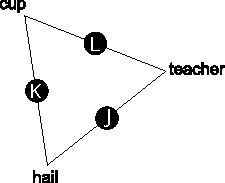
\includegraphics[]{images/triadExample.pdf}
\caption{\small{Example triad stimulus used in Experiment 1, showing English translations of the Dutch words used. If the participant believed that \stimulus{teacher} and \stimulus{cup} are the most related pair, they pressed the \textit{L} key.}}
\label{figure:ExampleTriad}
\end{figure}


\subsubsection{Procedure}
On each trial, three words were presented at the corners of an equilateral triangle, as shown in Figure~\ref{figure:ExampleTriad}. Each of the words was randomly allocated to one of the corners. In addition, the orientation of the triangle was randomized for each participant by rotating a triangle with one of its sides orthogonal to the screen in 20 degree steps (20, 40, 60 etc.) resulting in an orientation exemplified in Figure ~\ref{figure:ExampleTriad} which remained constant across all trials. During each trial, a red circle appeared in the centre of the triad. When the subject pressed the space bar, the word were shown at the corners of the triangle and the fixation circle turned green.

The instructions were accompanied with an illustration similar to Figure ~\ref{figure:ExampleTriad} and consisted of the following text (translated from Dutch):

\textit{In this study we want to investigate to what degree Dutch words can be considered related.
We will present a triangle on the screen with a red circle in the middle.
Press the space key to show the word. Next, three words will be displayed which represent three possible pairs. Press J, K, or L to select the most related pair. Note that the goal is to evaluate the meaning of these words and not the similarity between other things like letters or rhyme.
Think of relatedness in a broad sense.
Example 1.  \stimulus{cold} - \stimulus{hot} - \stimulus{square}. Here the first two words are related.
Example 2.  \stimulus{moist} - \stimulus{cold} - \stimulus{cool}. Here the last two words are related.
For some combinations the relatedness can be very weak. In these situations it might not be easy to choose a related pair. Even then, try to make a decision based on which words fit together based on what you think.}

The participants were asked to focus on the meaning of words rather than their orthographic similarity or phonological relatedness, and were asked to do their best even if the task seemed difficult. Also note that the first example contained an antonym, to inform the participants we cared about relatedness and not strict similarity. Responses were registered using a computer keyboard. In addition to the preference choice, decision latencies were also registered. At the beginning of each trial, the triad triangle was presented without any words displayed, until the participant pressed the space bar. When the space bar was pressed, the words were revealed and the circles shown in Figure \ref{figure:ExampleTriad} were labeled with the letters \textit{J}, \textit{K} and \textit{L}. Participants responded by pressing the appropriate letter key on an AZERTY keyboard. The task took less than 15 minutes to complete.


\subsection{Results and Discussion}

The choice preferences revealed a surprising degree of agreement among participants. If people's preferences were truly idiosyncratic, then we should expect that all responses should be equally plausible, and for very large samples, the choice frequencies should be roughly 33\% for all items. Because the modal frequency is by definition the largest of the observed frequencies, its expected value is slightly higher than 0.33 even when the choices are purely random.\footnote{\hspace{0.1cm}Calculating the exact number is slightly complicated because the extent of this bias depends on the sample size. If there were only a total of 10 observations, the expected value of the modal proportion is 0.49. When the sample size rises to 100 the expected value drops to 0.38, and by the time N=1000 it falls to 0.35. Our hypothesis tests take this into account. Our tests explicitly calculate the sampling distribution for the modal frequency, and do not literally test the modal frequencies against a value of 0.33. The R functions that we used to compute these probabilities and the rest of the statistical testing machinery are included in the additional materials} The observed pattern of responses is very different: in most cases there was a clear preference for one of the three options. This is illustrated in Figure~\ref{figure:RemoteTriadHistogram}, which plots a histogram of the modal choice frequencies across all 100 triads for 32 participants. The median value of the modal choice frequency is 0.63, which suggests that many preferences are above the expected modal frequency at chance level of 0.47.

To test whether these preference proportions are due to chance, we calculated Bayes factors for the largest mode (i.e., the most popular choice) and the goodness of fit for all three choice proportions.\footnote{\hspace{0.1cm}Note that these tests tend to be more conservative than frequentist versions based on permutation tests for the mode and $\chi^2$ for the overall goodness of fit reported for a pilot of these data in \textcite{DeDeyne2012Weak}. However, across all experiments reported here, the same qualitative results were obtained.}  The first test considers the presence of a suspiciously large mode and the results are shown in the left panel of Figure~\ref{figure:Exp1GOFTest}. Using a Bayes factor threshold (BF) of $\geq$ 3:1, ``modest evidence''  of such a mode was present for 67 of the 100 triads. Under a more stringent threshold (BF $\geq$ 10:1) evidence was found for 60 of the 100 triads, and under a very stringent threshold (BF $\geq$ 100:1) evidence was present for 47 of the 100 triads.
The second test, which considers goodness of fit for the choice distribution over the three alternatives, is consistent with these results. The results are displayed on the right panel of Figure~\ref{figure:Exp1GOFTest}. The Bayes factor reached the ``modest evidence'' threshold (BF $\geq$ 3:1) for 77 of the 100 triads, the more stringent  (BF $\geq$ 10:1) threshold for 69 of the 100 triads, and the very stringent (BF $\geq$ 100:1) threshold for 52 of the 100 triads.


\begin{figure}[t]
\begin{center}
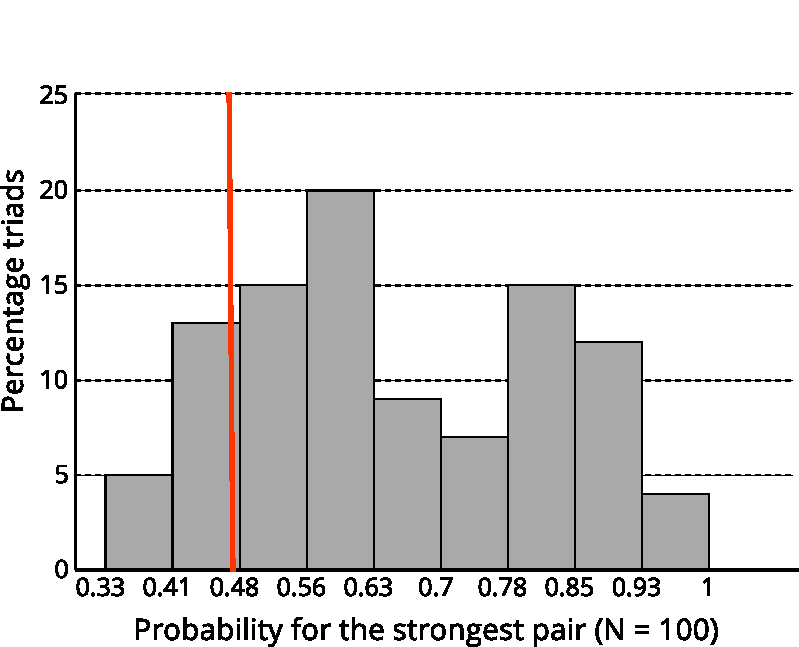
\includegraphics[width=9cm]{images/Exp1Histogram.pdf}
\caption{\small{Distribution of the modal responses (i.e., the most frequently chosen pair) based on the 100 triads in Experiment 1. If preferences were truly idiosyncratic, one would expect that choice frequencies should be around 47\% for all or most items with a sample size of 32 judgments. This is indicated by the vertical line in the Figure. That they are not is evidence that there is more agreement in these weak similarity judgments than one would expect by chance.}}
\label{figure:RemoteTriadHistogram}
\end{center}
\end{figure}

What regularities are people picking up on when they all select the same modal response? Examining individual triads is, unfortunately, not very helpful. For instance, the triad (\stimulus{butter}, \stimulus{train}, \stimulus{saddle}) was one that yielded strong evidence for a suspiciously large mode (most people said that \stimulus{train} and \stimulus{saddle} were most similar). One can always come up with post-hoc justifications of this choice -- perhaps it is because they both are thematically related to something involving transportation? perhaps because they are similar in size? -- but these have the flavor of ``just-so'' stories. It is also difficult to see how to generalize inferences about one triad to another: the first triad reveals little about why most people said that \stimulus{hyena} and \stimulus{somersault} were more similar in the triad (\stimulus{hyena}, \stimulus{somersault}, \stimulus{radish}). The additional three experiments in this paper are designed to more rigorously explore the question of what people are doing when they agree on weak similarities.

\begin{figure}[t]
  \centering
  \subfigure{
    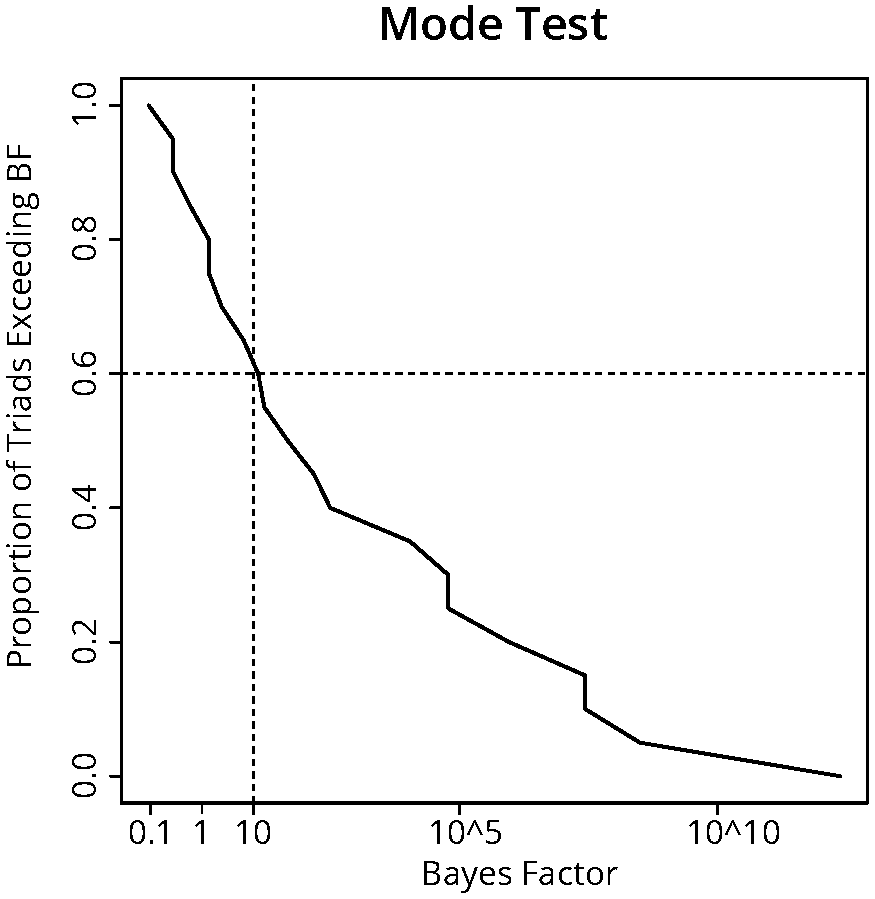
\includegraphics[width=7.3cm]{images/Exp1Mode.pdf}

    \label{figure:Exp1ModeTest}
    }
  \subfigure{
    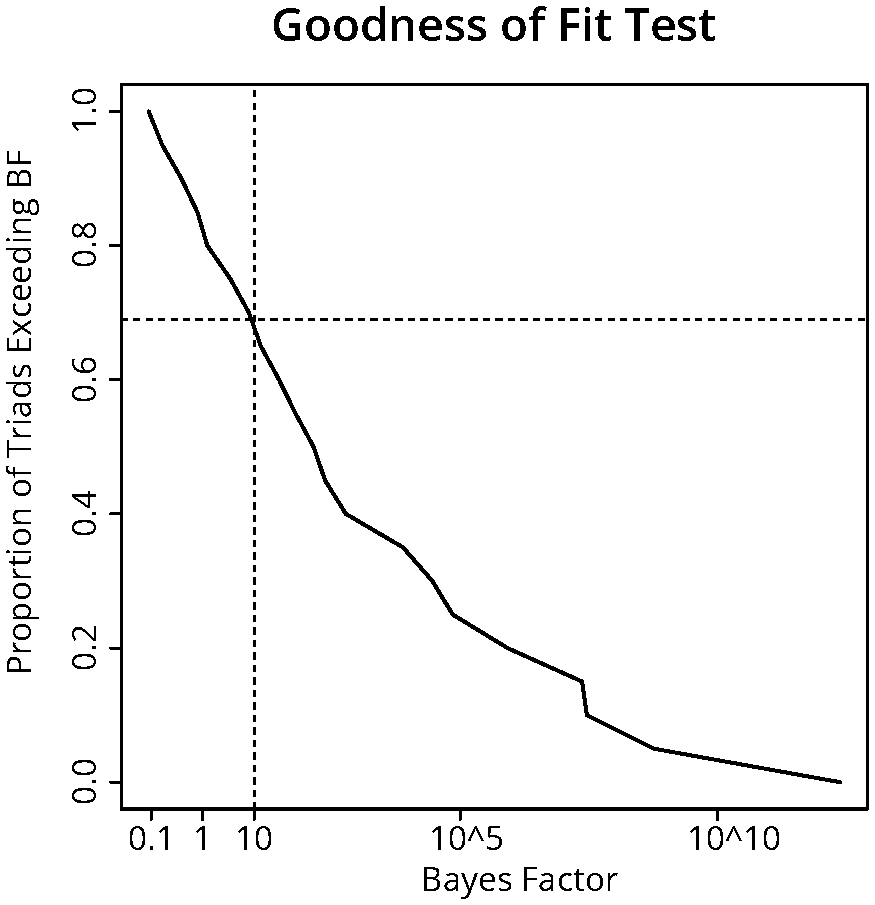
\includegraphics[width=7.3cm]{images/Exp1GOF.pdf}
    \label{figure:Exp1GOFTest}
    }
  \caption{\small{Experiment 1 Bayes Factors for the Mode (left Figure a) and the Goodness of Fit (right Figure b) for the three choices. Preferences on the right of the dotted vertical line indicates reliable evidence (BF > 10). In both cases, around two-thirds of the trials showed reliable evidence for a suspiciously large mode (representing more-than-expected agreement about which two items of a triad are more similar).}}
\end{figure}

\bigskip

\section{Experiments 2-4: Exploring the structure of weak similarity}

In light of the results from Experiment 1, it seems clear that there is some structure or some source of regularity underpinning the judgments people make about weakly related items. Experiments 2 through 4 are designed to further explore the nature of that structure. Experiment 2 constructs a clustering solution based on a small subset of items; the resulting structure helps to highlight the root and nature of the weak similarities. Experiment 3 explores the reasons that people give when asked to justify their choices. Finally, Experiment 4 provides a point of comparison by investigating people's judgments about strongly related items using the same experimental paradigm.



\subsection{Experiment 2: How is weak similarity organized?}

The results from Experiment 1 suggest that there is something non-arbitrary about the manner in which people perceive similarities between very different entities. However, it does not provide much of an insight into what those regularities might be. Choices might rely heavily on broad ontological distinctions such as living/nonliving \parencite[see e.g.,][]{Tallent2001,Garrard2001}, or they might rely on valence information \parencite[see e.g.,][]{Deese1965,DeDeyne2013}, or many other possibilities besides.  With this in mind, Experiment 2 adopts an exploratory approach. Using the same triadic choice task we calculate all pairwise similarities among a subset of the words and use a hierarchical tree to visualize the structure that emerges.\footnote{\hspace{0.1cm}We also considered a multidimensional scaling approach, but this produced far less satisfactory results.}

\subsection{Method}
\subsubsection{Participants} A total of 120 native Dutch speaking psychology students (92 females, 28 males, mean age of 19 years old, $SD$ = 1.61) participated in exchange for course credit. Following the same exclusion criteria as Experiment 1, a total of three participants were removed.

\subsubsection{Stimuli}

This task used a set of 25 nouns varying in degree of abstractness, listed in Appendix~\ref{table:AppendixBIBD}. Some belonged to natural categories and others to artifact categories. For 25 stimuli, there are $(_{\hspace*{2pt}2}^{25}) = 300$ unique pairs and $(_{\hspace*{2pt}3}^{25}) = 2,300$ unique triads. Each participant provided preferences for 100 of these triads. We used a balanced incomplete block design \parencite[see,][]{Burton1976} to ensure that all triads appeared with similar frequency across the whole experiment. Overall, 400 of the 2,300 possible unique triads were tested. To ensure overlap between participants, these 400 triads were divided into four sets of 100 triads each (where each set was judged by 30 participants). Within a set of 100 triads, each stimulus occurred 12 times in combination with two other words. This design ensured both that there was substantial overlap between the items participants saw, while at the same time reflecting a reasonable sample of the set of logically possible triads.


\subsubsection{Procedure} The procedure was identical to Experiment 1.

\subsection{Results and Discussion}
As in Experiment 1, people showed consistent preferences in their choices.\footnote{\hspace{0.1cm} The qualitative shape of the distribution of modal frequencies in Experiments 2, 3 and 4 is essentially identical to the pattern from Experiment 1 shown in Figure~\ref{figure:RemoteTriadHistogram}. To avoid repetition we have omitted the corresponding plots for the later experiments.}
The test of suspiciously large modes resulted in qualitatively similar, though somewhat attenuated, results as Experiment 1. There was modest evidence of suspiciously large modes (BF $\geq$  3:1) for 238 of the 400 triads, more stringent evidence (BF $\geq$ 10:1 ) for 178 of the 400 triads, and very stringent evidence (BF  $\geq$ 100:1) for 123 of the 400 triads. Similarly, the goodness of fit test for all preferences under a modest threshold resulted in evidence for 247 of the 400 triads, a more stringent threshold for 201 of the 400 triads, and a very stringent threshold for 151 of the 400 triads. Altogether these results replicate those of Experiment 1: most triads were only weakly related, yet people substantially agreed about which pairs belong together.

Since these stimuli covered a variety of words (including abstract, natural kind and artifact concepts), it is possible to test whether a simple heuristic might explain people's choices. If so, broad distinctions should become apparent by inspecting the similarity structure in the preference data. In order to visualize the structure implied by participant choices we constructed a matrix of pairwise similarities $\mathbf{S}$. The similarity between any two words was calculated by counting the number of times that pair of words was chosen as the most similar, and dividing it by the number of occasions in which that pair was presented as part of a triad.
Next, we extracted an additive tree representation using the algorithm proposed by \textcite{Lee1999}. This algorithm allows us to estimate the number of internal nodes based on BIC complexity rather than determining this number {\it a priori}.\footnote{\hspace{0.1cm} As did \textcite{Lee1999}, we varied the precision between values of 0.1, 0.2 and 0.3 to estimate the BIC and decide on the number of internal nodes; the specific value of precision did not impact the main results.}

The best tree model (i.e., the lowest BIC) consisted of seven internal nodes and is shown in Figure~\ref{fig:MDSClusteringSolution}. The tree distances correctly identify the modal response in 310 out of 400 cases. The variance accounted for by this model was 45\%, which is fairly low (around 70\% is more typical). This contrasts with the findings for more homogeneous domains, like animals \parencite{Lee1999}, and suggests that the similarity structure in our data isn't easily captured.


The tree structure is fairly sensible, creating groups of entities corresponding to superordinate categories such as animals (\stimulus{poodle}, \stimulus{worm}, \stimulus{tiger}, \stimulus{camel}, \stimulus{swallow} and \stimulus{eel}) and geography (\stimulus{mountain}, \stimulus{field}). The tree also picks out categories of items that share a common very salient feature (e.g., a \stimulus{bomb} and \stimulus{thunder} are both loud and violent). To the extent that people's choices reflect these categories, the results seem unremarkable: it is hardly a surprise that people would decide that \stimulus{tigers} and \stimulus{camels} are more similar to each other than either is to \stimulus{butter}.

However, people also often rely on thematic and {\it ad hoc} connections when judging similarities, even though thematic relations in this study emerged by coincidence from the pairings of a small and diverse set of words. Such thematic connections are only sometimes captured by the additive tree solution. Some connections are apparent in the tree: \stimulus{breath} is especially important to an \stimulus{athlete}, the sound of \stimulus{thunder} can be loud like the explosion of a \stimulus{bomb}, a \stimulus{crust} goes in the \stimulus{garbage}, and so on. Yet many others are not: for instance, for the  triad \stimulus{field -- bomb -- worm}, participants have a clear preference for \stimulus{field -- worm}, whereas the tree suggests a grouping of \stimulus{field -- bomb}.

In general, while capturing the broad distinctions such as animals or artifacts, the tree fails to capture many of the instances where people rely on a thematic relation between a living thing and artifact or abstract concept. This suggests, in keeping with other work \parencite{Lin2001,EstesGolonka2011}, a preference for thematic relatedness even if a presumably more simple taxonomic relationship exists.
Overall, between the relatively poor fit of the additive tree representation and its failure to identify many thematic relationships, this experiment suggests that a small set of heuristic principles such as valence or living vs natural kinds cannot fully account for weak similarity judgments in the triadic preference task (although they may partially do so).



\begin{figure}[t]
\centering
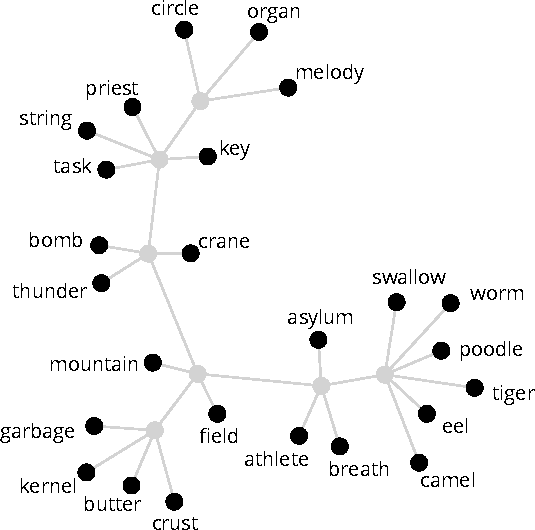
\includegraphics[width=7cm]{images/addTreeNodes10.pdf}
\caption{\small{Visualization of the additive tree representation using 7 internal nodes based on the relatedness choices in Experiment 2.}}
\label{fig:MDSClusteringSolution}
\end{figure}



\subsection{Experiment 3: How do people explain their choices?}

In light of the results from Experiment 2, it seems clear that at least part of how people make judgments about randomly chosen items is to pick out items that belong to the same broad domain. However, it is also clear that this simple heuristic fails to capture a large proportion of the variance in their judgments. What else are they doing, and why? To address this question, Experiment 3 showed people stimuli from the same broad domain, thus eliminating the ability to use broad domain to drive decisions. We also asked them to provide reasons for their choices. Do people who make the same choices tend to offer the same reasons for those choices? Or do people find it difficult to explain why they made their decisions?

\subsection{Method}
\subsubsection{Participants} A total of 66 native Dutch speaking psychology students (58 females, 8 males, average age 19, $SD$ = 1.0) participated in exchange for course credit.

\subsubsection{Stimuli} The triads were constructed using the stimuli from \textcite{DeDeyne2008}, which consisted of a set of animals containing five categories (birds, fish, insects, mammals and reptiles) and a set of artifacts containing six categories (clothing, kitchen utensils, musical instruments, tools, vehicles and weapons). Using these items, a set of 63 triads were constructed, 28 for the animals and 35 for the artifacts. These triads were constructed such that no item appeared in more than one triad, and no triad contained items from the same category. That is, \stimulus{monkey}--\stimulus{trout}--\stimulus{sparrow} is an allowed triad, but \stimulus{monkey}--\stimulus{dog}--\stimulus{sparrow} would not be allowed because it contains two mammals. To match the length of the previous experiments and to decrease strategic processing that could result from the relatively small number of categories, a total of 37 triads were randomly selected from Experiment 1.
The stimuli used in this experiment are presented in Appendix~\ref{Appendix:DomainTriads}.

\subsubsection{Procedure} The first part of the experiment was a triadic choice task identical to Experiments 1 and 2. It  was completed by all participants. The second part was presented only to 20 of these participants: after completing the triad judgments they were shown the same triads with their previous choices highlighted and asked to provide an explanation (free response) for why they thought the chosen pair was more related.

\subsection{Results and Discussion}
Consistent with Experiments 1 and 2, people's choices were non-arbitrary. A test for suspiciously large modes found modest evidence for 73 of the 100 triads (BF $\geq$ 3:1), 68 out of 100 triads for a more stringent threshold (BF $\geq$ 10:1) and 58 out of 100 triads under a very stringent threshold (BF $\geq$ 100:1). For the goodness of fit test, modest evidence was found for 79 out of 100 triads (BF $\geq$ 3:1), 74 out of 100 triads under the more stringent threshold (BF $\geq$ 10:1) and 67 out of 100 triads under the very stringent threshold (BF $\geq$ 100:1).

The same pattern of results was obtained comparing the animals, artifacts and random triads that were part of this experiment. For example the goodness of fit test under a stringent threshold showed comparable evidence for random triads (27 out of 32 triads) and animal triads (22 out of 28) which in both cases was a bit more extensive than the results for artifacts (25 out of 40 triads).

Next, we evaluated the interpretations participants made for their own preferences for each of the 100 triads.
Overall, people were able to provide a justification 86\% of the time, and among the reasons offered there appeared to be a substantial amount of agreement across participants. For instance, most people judged \stimulus{soup} and \stimulus{diarrhea} to be more similar to each other than either is to \stimulus{dress}. The reasons offered tended to be very similar as well, including justifications such as \textit{both are running}, \textit{running}, \textit{fluid}, \textit{both are fluid} and \textit{watery}. To quantify this intuition, two independent raters were asked to sort the participant responses into groups of similar reasons. The raw agreement between the two raters was 81\% ($SD = 13\%$), corresponding to a substantial Cohen's kappa ($\kappa  = .759$, $z = 51.2$, $p < .001$).
According to Rater 1, there were an average of 4.99 distinct explanations given for any given triad ($SD=1.8$), whereas for Rater 2 the average was 3.13 ($SD=1.86$). However, these numbers overstate the heterogeneity of people's responses as many of these explanations occur only once whereas others can be highly frequent.


We also assessed the homogeneity of people's explanations for a response by calculating the modal response frequency. If this is higher than 1, it would suggest that participants agree upon the underlying explanations  rather than making completely idiosyncratic response interpretations. This was calculated averaged over triads for each of the three choice preferences and excluding the ``no relation'' explanations. For Rater 1, the modal or most frequent interpretation was 6  ($SD = 3.52$), 2.31 ($SD = 3.52$) for the second most frequent choice preference and 1.1  ($SD = 0.9$) for the least frequent choice preference.
For Rater 2, the modal interpretation was 7.16 ($SD = 3.92$) for the most frequent choice preference, 2.51 ($SD = 1.68$) for the second most frequent choice preference and 1.22 ($SD = 1.00$) for the least frequent choice preference. Obviously these values are smaller for the less frequent response preferences as we already observed that these frequencies are skewed.
Focusing just on the most frequent choice preferences, distinguishing the remote animal, artifact and random triads from Experiment 1, showed that the nature of the triad does not affect the results strongly, and if anything more homogeneous explanations were given for the random triads from Experiment 1 (modal frequencies being 6.25, 4.63 and 7.50 for respectively animals, artifacts and random triads for Rater 1 and 6.96, 5.90 and 8.91 for animals, artifacts and random triads for Rater 2).

Regardless of the nature of the triad or the choice participants made in the first part of the experiment, or the rater, the modal frequency is higher compared to complete idiosyncratic explanations.
In conclusion, this extends our previous finding, namely that people show considerable agreement for their triadic choices, to agreement for the interpretation of their choices.


A final way to evaluate the nature of the weak similarities is to apply a semantic coding scheme to people's explanations of why they chose a given pair. The coding scheme was based on a simplified version of the Wu and Barsalou ontology  \parencite{Wu2009,McRae2005,Brainerd2008,Santos2011} which was later adapted for word associations and as described in \textcite{DeDeyne2008b}. We are interested only in the five main distinctions in this ontology defined in Appendix~\ref{Appendix:SemanticOntology}. This means that for example only a taxonomic relation is coded, rather than specifying different taxonomic relations (superordinates, coordinates or subordinates).  This resulted in five major types of explanations: taxonomic (e.g., for the chosen pair \stimulus{guitar}-\stimulus{spoon} and the explanation \textit{both are objects}),  lexical  (e.g., \stimulus{caravan}-\stimulus{cello}, \textit{both start with C}), thematic (e.g., \stimulus{vulture}-\stimulus{tiger}, \textit{live in Africa}), feature (e.g., \stimulus{blouse}-\stimulus{towel}, \textit{made of fabric}), and valence  (e.g., \stimulus{witch}-\stimulus{fat}, \textit{bad things}).


The results are shown in Figure~\ref{fig:SemanticCoding}. Regardless of the type of triads, the majority of the explanations were thematic, followed by shared features and taxonomic explanations. These results are consistent with Experiment 2; both indicate that many people relied on thematic relationships when judging these similarities. Moreover, the results also closely follow previous studies where word association responses were classified according to the same ontology and the same ordering for the three major classes (Thematic > Feature > Taxonomic) was obtained \parencite{DeDeyne2008b}.
Further examining the different types of triads shows very similar results for both animal and artifact triads.
The only notable difference was the higher percentage of thematic explanations for the random triads. Potentially this reflects the larger distances between words in these triads which makes it harder to come up with shared features or a shared taxonomic level.
Most importantly, the types of explanations for remotely related items cannot be accounted for by general factors like shared lexical valence information. Taxonomy could in theory also explain distances between any arbitrary pair of words \parencite[cf. WordNET,][]{Fellbaum1998}, but at least at a subjective level, this information was less prominent. Instead, agreement seems to be explained mostly in terms of a shared theme, a point which we will revisit in the General Discussion.

\begin{figure}
\centering
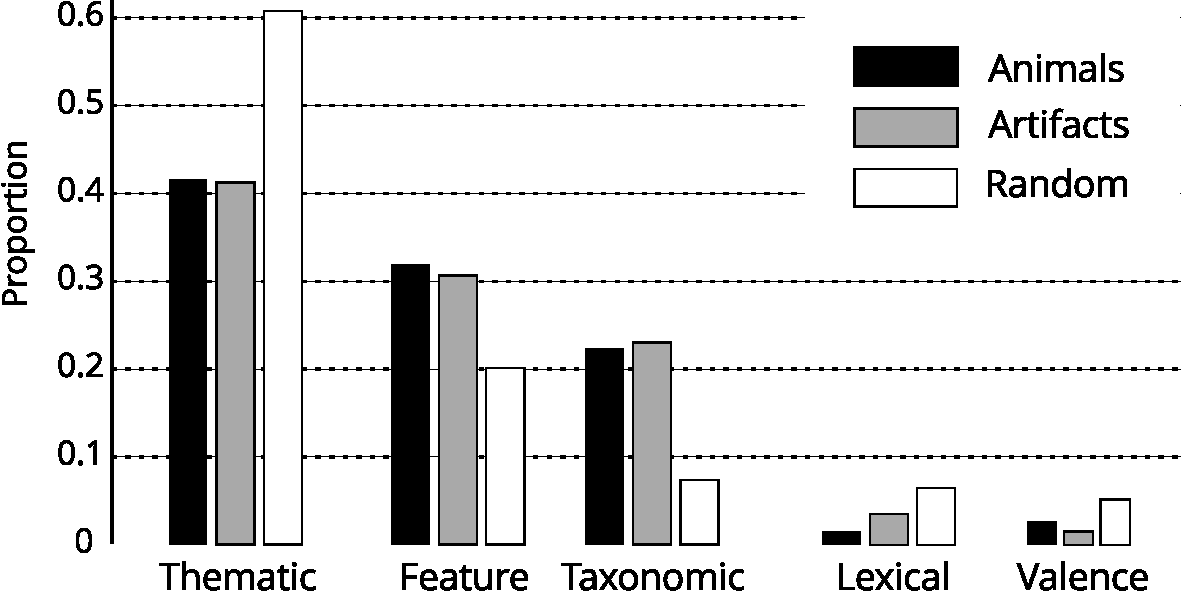
\includegraphics[width=11cm]{images/Exp4SemanticCodingSplitByType.pdf}
\caption{\small{Coding of post-hoc participant explanations using the semantic ontology in Experiment 3 for animal, artifact and random triads.}}
\label{fig:SemanticCoding}
\end{figure}


\subsection{Experiment 4: Comparison to strong similarities}

In Experiments 1 and 2 we considered genuinely ``weak'' similarities, with words selected largely at random from Dutch nouns. Experiment 3 incorporated somewhat stronger similarities in which all items within a triad belonged to the same general domain (e.g., animals). In Experiment 4, we make the constraint even stronger by restricting items to belong to the same basic level category (e.g., birds). Doing so ensures that, across all four experiments, we have a broad range of similarities to consider when fitting theoretical models to the data in the second part of the paper.


\subsection{Method}
\subsubsection{Participants} A total of 51 native Dutch speaking psychology students (40 females, 11 males) participated in exchange for course credit. The average age was 18 years (SD = 0.8). Using the same criteria as in the previous experiments, two participants were removed.

\subsubsection{Stimuli}
A total of 100 stimuli were selected from the concept norms in \textcite{DeDeyne2008} for five animal categories (bird, fish, insects, mammals, and reptiles), six artifact categories (clothing, kitchen utensils, musical instruments, tools, vehicles, and weapons), two food categories (fruits, vegetables), and two activity categories (professions and sports). Each item in a triad occurred only once in the stimulus set, and all triads contained items from the same basic level.  A list of these stimuli can be found in Appendix~\ref{table:AppendixBasicLevelTriads}.


\subsubsection{Procedure} The procedure and test conditions were identical to Experiment 1.

\subsection{Results and Discussion}

As in the other experiments, people showed a strong degree of agreement.  For the test of suspiciously large modes and using the same qualitative interpretation of BF, we found modest evidence (BF $\geq$ 3:1) for 85 out of 100 triads, 76 of the 100 triads under a more stringent threshold (BF $\geq$ 10:1) and 68 out of 100 under a very stringent threshold (BF $\geq$ 100:1).
For the goodness of fit test modest evidence was found for 88 of the 100 triads, evidence for 83 out of 100 triads under more stringent criteria and evidence for 74 of the 100 triads under very stringent criteria.

Since the main purpose of this experiment is to explore how the model presented in the next section predicts people's judgments at different scales (from remote to within-domain to within-category), we defer further discussion of the experiment to the model performance. First we explain our model for weak similarity in the next section.



%%%%%%%%%%%%%%%%%%%%%%% THE MODEL ITSELF %%%%%%%%%%%%%%%%%%%%%%%

\section{A network model for weak similarities}
The most surprising characteristic of our data is the fact that people have such strong agreement regarding weak relationships. When asked to select the most similar pair from an apparently arbitrary triad such as \stimulus{cup}--\stimulus{hail}--\stimulus{teacher}, people do not choose randomly nor do they choose idiosyncratically. In fact, the extent of this agreement across people is approximately the same magnitude when the relationships are weak as it is when they are strong. In Experiments 1 and 2 where the similarities were weakest the proportion of people choosing the most common response was 63\% and 59\% respectively. Forcing all items to belong to the same domain (Experiment 3) made little difference, with the agreement rate being 59\%. A more extreme manipulation in which all items in a triad belonged to the same basic level category (Experiment 4) only produced a modest effect, with the agreement rate being 70\%.

Given that there is consistency among people's responses, it is natural to ask whether this consistency is {\it predictable}. Is it possible to construct a semantic model that produces the same choices that people do? In this section we show that a simple spreading activation mechanism within a semantic network model naturally produces the same pattern of behavior as human subjects, whereas simpler models that rely on shared features (indicated by common associative neighbors) are unable to do so.


\subsection{Approximating semantic networks with word associations}

The approach we take to modeling weak similarity is a fairly standard spreading activation model \parencite{Collins1969,Collins1975}. In this approach, concepts are represented by nodes in a semantic network, and edges connect concepts that are directly related to one another. When one concept is activated, this activation extends to linked concepts.
Network models are widely used within cognitive science \parencite{Hutchinson1989,Schvaneveldt1988,Sloman1998b,DeDeyne2008a,DeDeyne2011,Steyvers2005,Hills2009longitudinal,Vitevitch2008,Baronchelli2013}, and while they are by no means the only method for describing how word meaning could be represented \parencite[e.g.,][]{Landauer1997,Griffiths2007,Jones2007,NavarroGriffiths2008,NavarroLee2004,Tversky1977} they strike the balance between interpretability and flexibility appropriate for the current purposes.


From a methodological standpoint, the critical question is how the semantic network should be approximated. One prominent approach is to take word co-occurrence information and apply statistical tools to extract the latent semantic structure \parencite[e.g.,][]{Landauer1997,Griffiths2007}. The difficulty with this approach is that lexical co-occurrence reflects many other factors besides semantic relationships: for example, pragmatic communicative rules ensure that people say ``green banana'' to specify that a banana is green, but do not say ``yellow banana'' when a banana is yellow. Notwithstanding the fact that lexical co-occurrence data has many virtues \parencite{Jones2014}, the relation between word association responses (which do not have these pragmatic constraints) and text-coocurrence is moderate at best \parencite{Szalay1978,DeDeyne2013b} and it is not clear how word co-occurrences are encoded. For these reasons lexical co-occurence does not constitute the purest measure of the associations that exist between concepts although we revisit this alternative in the general discussion.


As argued previously \parencite[e.g.,][]{DeDeyne2014CorpusSize}, a more direct approach is to use (observed) word association data as a proxy for (latent) semantic associations. In this approach, we construct a weighted adjacency matrix $\mathbf{G}$ in which the value of $g_{ij}$ counts the number of times that word $j$ is given as an associate of word $i$. In order to make this work, a large data base of word associations is required. For our application, the word association data come from a study consisting of $N$ = 12,428 cue words and over 3 million responses, in which each participant was given a short list of cue words and asked to generate three different responses to each cue \parencite[see][]{DeDeyne2008a,DeDeyne2011}.

Using these data, we can construct two qualitatively different graphs, denoted  $\mathbf{G}_1$ and $\mathbf{G}_{123}$. For both graphs, we extracted the largest component by only keeping those cues that were also given at least once as a response. This way all words can be reached by both in- and out-going links. The graph $\mathbf{G}_1$ only counts the  first response given by the participant.
Its largest component includes $N$ = 11,957 nodes and only 0.23\% of the possible links. The graph based on $\mathbf{G}_1$ is the more conventional approach, and its sparsity is comparable with previous word association studies \parencite{Nelson2004}. The second graph, $\mathbf{G}_{123}$ counts all three responses. Because it is based on more responses, the largest component used to construct $\mathbf{G}_{123}$ is somewhat denser: $\mathbf{G}_{123}$ included $N$ = 12,408 nodes and 0.64\% of possible links.

Previous work on associative strenght indicates that the frequency of responses itself does not reflect a direct measure of associative strength of the responses, but a nonlinear function describes the relation between strength and response frequeny \parencite[see p 10][]{Deese1965}. In this study, associative strength between a cue and response was derived by calculating the conditional probability of a response given a cue. This way, each cue had the same  marginal probability. In other words, the total strength of each row of $\mathbf{P}$ sums to one. Next, we calculated associative strength as the {\it positive pointwise mutual information measure} \parencite[see][]{Jurafsky2008}.
\begin{equation}
\mbox{PMI}^+(p_{i|j}) = max\left(0,log_2 \left(\frac{p(i|j)}{n \sum_j p(i|j)} \right)\right)
\end{equation}
In this equation, the denominator takes into account how often a response is given for all cues.
This way, responses that are given very frequently for many cues are considered less informative than responses that are given for only a small number of cues. Similar to text-corpus based studies, we expect this approach to positively affect the performance in semantic tasks \parencite{Bullinaria2007}, and as we will see later on, also allows us to limit the number of links along which information spreads in the graph.


\subsection{Using semantic networks to predict weak similarity}
Similar to previous lexico-semantic approaches derived from text \parencite{Recchia2009} or word associations \parencite{Deese1965,BorgeHolthoeferArenas2010,Steyvers2004,DeDeyne2009} the similarity between pairs of words is expressed as the distributional overlap of word co-occurrences or shared neighbors in a semantic graph.
Focusing on the case of word associations, this means that words with a similar distribution of responses will have similar meanings. Typically the number of different associations is limited, which means that for any arbitrary pair of words, there simply is no overlap or it is limited to just a few shared responses.
Here we propose that additional information can be inferred from the indirect paths between words in the network, which might still result in meaningful similarity indices even if two words do not share any common neighbors.


Given that ``association'' and ``similarity'' are highly related measures, it seems natural to expect that focusing on a distributional measure derived from shared neighbors would do a good job of predicting strong similarities, such as that between \stimulus{lion} and \stimulus{tiger}. These are highly similar concepts,  with many properties in common. It seems much less plausible to believe that it would account for weak relationships. In Experiment 2, for example, we discussed the similarity between \stimulus{athlete} and \stimulus{breath} that emerges from the data. This similarity is easy to spot even though these are not directly linked. Yet it is not difficult to {\it construct} a relationship between the two. An athlete does exercise, and doing exercise will cause one to start panting and lose one's breath. This line of reasoning would map onto an associative chain such as \stimulus{athlete} $\rightarrow$ \stimulus{exercise} $\rightarrow$ \stimulus{pant} $\rightarrow$ \stimulus{breath}. Although there is no  direct line between the two concepts, it is easy to see how a spreading activation mechanism \parencite[e.g.,][]{Collins1969} would uncover such a connection, and thereby be able to capture the relationship between these items. More generally, by exploiting the structure of the semantic network, a spreading activation model might be able to infer additional information through indirect links which might capture answers similar to humans when presented with an arbitrary triad such as \stimulus{cup}--\stimulus{hail}--\stimulus{teacher}. In particular, we expect that the distributional overlap consisting of not only directly shared associations but also indirect neighbors that are not shared is considered when evaluating remote triads.


To quantify this idea we adapt the Katz index \parencite{Katz1953} which closely resembles a decaying  random walk approach given the fact that rows in $\mathbf{P}$ sum to 1 and thus corresponds to a random walk transition matrix \parencite[see also][]{AbbottAusterweil2015,BorgeHolthoeferArenas2010,Griffiths2007b,Kemeny1976,Leicht2006}. When a node is activated it starts a random walk (or many such walks) through the graph, activating nodes that the walk passes through. From this perspective, similarity is related to the number and length of the paths through the network that connect two nodes. If there are many short paths that connect two nodes, then it is easy for a random walk through the graph to start at one node and end at the other; these nodes are then inferred and added to the distribution over which to calculate similarity. Formally, the measure is specified by beginning with the adjacency matrix containing associative strengths $\mathbf{P}$ introduced before.
It is useful to first consider an iterative procedure to derive the random walk similarities as follows \parencite{Newman2010}. Consider a walk of a maximum length $r = 3$ where $\mathbf{I}$ is the identity matrix and the damping parameter $\alpha < 1$ governs the extent to which similarity scores are dominated by short paths or by longer paths:


\begin{equation}
\begin{array}{lcl}
\mathbf{G_{rw}}^{(r=1)} & = & \mathbf{I}\\
\mathbf{G_{rw}}^{(r=2)} & = & \alpha \mathbf{P} + \mathbf{I}\\
\mathbf{G_{rw}}^{(r=3)} & = & \alpha^2\mathbf{P}^2 + \alpha\mathbf{P} + \mathbf{I}\\
\end{array}
 \label{equation_iteration}
\end{equation}

During each iteration, indirect links reflecting paths of length $r$ are added to the graphs.
Longer paths receive lower weights because of the exponent $r$ of $\alpha$.
The same expression can also be computed more directly by taking the inverse of $\mathbf{P}$ and considering the limit case with infinity long paths:

\begin{equation}
\begin{array}{lcl}
\mathbf{G_{rw}}  = \sum_{r =0}^{\infty}(\alpha\mathbf{P})^r  =   (\mathbf{I} - \alpha \mathbf{P}^{-1})
\end{array}
\label{equation_RW_algebraic}
\end{equation}

\noindent

Viewed in terms of the underlying random walk, the probability that the walk terminates (i.e., the spreading activation dies out) at any given time step is $1-\alpha$.\footnote{Equation \ref{equation_RW_algebraic} converges only for values of $\alpha < \frac{1}{\sigma_{max}\mathbf{P}}$ where $\sigma_{max}\mathbf{P}$ is the largest singular value. Given the fact that $\mathbf{P}$ is a transition matrix for the largest connected component of $\mathbf{G}$, $\sigma_{max}(\mathbf{P})$ always equals 1. For this reason only values of $\alpha$ larger than 0 and smaller than 1 will be considered.

} The probability of an associative chain surviving across $r$ links is thus $\alpha^r$. The smaller the value of $\alpha$, the larger the contribution made by very short paths. This ``decay'' parameter serves an important theoretical role. As noted by \textcite{Minkov2008}, if this parameter is omitted the model becomes vulnerable to one of the major criticisms of the spreading activation mechanism, namely the fact that the entire network is quickly activated \parencite[e.g.,][]{Ratcliff1994}.  Note that under this approach the path lengths can be asymmetric (i.e., $p(i|j) \neq p(j|i)$). At this point, the random walk graph $\mathbf{G}_{\textrm{rw}}$ combines paths of various lengths obtained from the random walk. However, these paths do not conform to the associative strength measure proposed earlier (rows do not sum to one and many paths occur for many cues and are therefore uninformative). To be able to compare the random-walk augmented $\mathbf{G}_{\textrm{rw}}$ with $\mathbf{P}$, we apply the positive pointwise mutual information measure $\mbox{PMI}^+$ transformation and normalize the values to conditional probabilities to derive $\mathbf{P}_{rw}$ from $\mathbf{G}_{rw}$.

 As before we consider the similarity between two words to be the cosine distance. In other words, two words are similar if they have a similar distribution of paths (now including indirect paths).
Since our experimental design forces the empirical similarities to be symmetric we use the average of $\mathbf{S}$ and $\mathbf{S}^T$ in our evaluations.\footnote{\hspace{0.1cm}For both the cosine and random walk similarity measures the computed similarity values for each triad are normalized to sum to 1. This allows the model predictions to be directly comparable to the empirical choice probabilities, which also sum to 1. This is equivalent to assuming that the network activation level corresponds to the response strength and using Luce's choice rule \parencite{Luce1959} to construct choice probabilities.}



\subsection{Illustrating the contribution of indirect paths and activation decay}
To illustrate how indirect paths are obtained, what the role of $\alpha$ is, and how it interacts with other aspects of our approach in more detail, we calculated the predicted links by the random walk procedure in Equation \ref{equation_RW_algebraic}. Consider the word \stimulus{tiger}. Participants will associate it with words like \stimulus{stripes}, \stimulus{wild}, \stimulus{animal}, \stimulus{zoo} and so on. The random walk process will infer additional indirect links as well, and depending on the value of $\alpha$, it will do so taking into account shorter or longer paths. At the same time, due to the small world properties of associative networks \parencite[see][]{Steyvers2005,DeDeyne2008b}, we know that the network is highly clustered around hubs (i.e. highly connected nodes like \stimulus{water},\stimulus{sun},\stimulus{good}, etc). A first consequence is that many paths go through these nodes and be quite similar regardless of the identity of the  cue. A second consequence is that given the short path lengths of the semantic network where each node can be reached in about three steps, the entire network quickly becomes activated.


\begin{table}[ht]
\centering
\caption{Top 10 novel indirect paths inferred for the word \stimulus{tiger} and various values of $\alpha$ for unweighted and $PMI^+$ weighted paths. The network density $D$ is indicated on the second row.}
\begin{small}
\label{my-label}
\begin{tabular}{cccclcccc}
\toprule
\multicolumn{4}{c}{Unweighted paths} &  & \multicolumn{4}{c}{Weighted paths} \\
\cline{1-4} \cline{6-9}
$\alpha = .25$ & $\alpha = .50$          & $\alpha = .75$   &   $\alpha = .95$         & &
$\alpha = .25$ & $\alpha = .50$          & $\alpha = .75$   &   $\alpha = .95$              \\
$D$  = 1.00   & $D$  = 1.00  & $D$  = 1.00 & $D$  = 1.00 & &
$D$  = 0.01   & $D$  = 0.03  & $D$  = 0.08 & $D$  = 0.10 \\
\midrule
animals & animals & animals & fun 		& & leopard & leopard   & leopard      	& lioness  \\
bear    & bear    & beast   & nice     	& & safari  & safari   & hyena   	& hyena        \\
safari  & beast   & bear    & comfy     & & bear    & hyena    & lioness 	& cougar       \\
beast   & safari  & dog     & warmth    & & zebra   & lioness  & safari  	& leopard      \\
leopard & leopard & safari  & friends  	& & giraffe & zebra    & zebra       & devour      \\
dog     & dog     & forest  & pleasure 	& &fox     & giraffe   & devour      & jungle      \\
fox     & fox     & leopard & love    	& &        & devour    & pheasant    & Jerry can   \\
ape     & rabbit  & fun     & enjoyable & &        & pheasant  & carnivore   & carbine     \\
wolf    & forest  & warmth  & enjoy 	& &        & carnivore & cougar      & pheasant    \\
rabbit  & jungle  & sun     & sun       & &        & jaguar    & bird of prey& bird of prey\\
\bottomrule
\end{tabular}
\end{small}
\label{Table:tiger}
\end{table}

At $\alpha = .95$, the unweighted paths become biased towards nodes that have high in-strength (i.e. weighted incoming links). In other words, the most highly weighted new links are strongly correlated with the most popular responses. In this example, $r(p(j|\mbox{\stimulus{tiger}}), p(j))$ = .83 for $\alpha$ = .95 and approaches 1 as $\alpha$ approaches 1, whereas for the weighted paths, such a bias is absent: $r(p(j|\mbox{\stimulus{tiger}}), p(j))$ = .02 for $\alpha = .95$.\footnote{This highlights the strong similarities to the PageRank measure:  $\mathbf{X}  =  (\mathbf{I} - \alpha \mathbf{P}^{-1})\mathbf{1}$. In other words, the PageRank measure reflects the centrality of a node as the weighted sum of all indirect paths it has \parencite{Page1998}.} The frequency bias is general and manifest at high $\alpha$-values in such a way that the contribution of the original cue node from which the walk departs becomes negligible. This frequency bias has been previously documented by \textcite{Newman2010} and often is countered by down-weighting the path weights as a function of the number of in- or out-going links.
Rather than simply dividing the weights by their total strength, we applied the same $PMI^+$ weighting function as before as it has the additional benefit of keeping the graph relatively sparse since only positive weights are added. To illustrate implications of this, we calculated the density of $\mathbf{G}_{\textrm{rw}}$ for the values of $\alpha$ in Table~\ref{Table:tiger} as well. Indeed, as can be seen from the last four columns of Table~\ref{Table:tiger}, the additional words activated for various values of $\alpha$ suggest a sensible result where the density of the network remains small and additional information can be inferred from a relatively small number of new paths.



\subsection{Deriving a network-based similarity measure}
So far we have shown that we can infer sensible links through a mechanism of spreading activation. Similar to other studies, we will first assume that the similarity between pairs of words is not reflected by the shortest path between two words, but by looking at the distributional overlap of the paths they share \parencite{BorgeHolthoeferArenas2010,Deese1965,DeDeyne2014CorpusSize}. Given a semantic network, how does one measure the distributional similarity between two entities? In this paper we consider the widely used cosine measure of similarity \parencite[e.g.,][]{Landauer1997,DeDeyne2014CorpusSize,Steyvers2004}, which measures the extent to which two nodes have the same neighbors. Two nodes that share no neighbors have a similarity of 0, and nodes that are linked to the exact same set of neighbors have similarity 1. Formally, the cosine measure is as follows. Each row of the original associative strength matrix $\mathbf{P}$ or the matrix with indirect paths $\mathbf{P}_{rw}$ is normalized by the $L_2$ norm, which gives us a $\mathbf{N}$ such that $n_{ij} = p_{ij} /\sqrt{\sum_{j} {p_{ij}}^2}$. The matrix of pairwise similarities $\mathbf{S}$ is given by

\begin{equation}
\mathbf{S} = \mathbf{N}\mathbf{N}^T
\end{equation}

\noindent
By normalizing the dot product by the $L_2$ norm it takes into account frequency differences that might exist between these distributions.

When no indirect paths are inferred through the random walk introduced before, this local shared neighbors similarity rule is very similar to the widely-used common features similarity model \parencite{Tversky1977}. The key thing to recognize is that it depends solely on the {\it local} structure of the graph: the similarities between two entities is assessed by looking only at the items to which they are immediately linked.
This simple measure does not rely on any deep structural characteristics of the network but provides a theoretically-important baseline. By relying only on the raw data itself, it provides a measure of the extent to which word association data are in fact ``similarity in different clothes.'' To the extent that the local cosine measure provides a good account of the similarity data, we might conclude that the word association task is just redescribing similarity, and the exercise of explaining one using the other is circular. Moreover, if it is the case that network similarity measures that rely on indirect paths cannot provide a better account for our data than the local cosine model, we should conclude that the semantic network formalism provides no added value, and the raw data are doing all the heavy explanatory work.

% TOT P 29
%%%%%%%%%%%%%%%%%%%%%%% FITTING THE DATA %%%%%%%%%%%%%%%%%%%%%%%

\section{How well does the network model perform?}

In this section we evaluate the performance of the network similarity model. In the first part we look at the performance of the cosine measure and the spreading activation measure for all four experiments, and show that -- as one might expect -- the cosine shared neighbor measure can account for strong but not weak similarities, whereas the spreading activation method accommodates both. We follow this with a consideration of the role played by the $\alpha$ parameter in controlling network similarities. Finally, we present a more detailed investigation that explores the qualitative difference between strong similarity and weak similarity by inferring which paths contribute most strongly to different kinds of judgment.

\subsection{Overall performance of different models}

To evaluate how well the remote triad choice preferences from our experiments can be captured using the semantic network models, we calculated the correlations between the network-derived similarities and the empirical choice preferences for all four experiments. In order to compare our approach to more traditional word association studies and investigate the role of network density, we compare the performance of these different measures when the network is constructed from only the first response given by each person (i.e., the graph $\mathbf{G}_1$) and when it is constructed using all responses (i.e., the graph $\mathbf{G}_{123}$). For all experiments, the $\alpha$ parameter for the random walk model was set at 0.75 as this provided good results regardless of nature of the task. A systematic evaluation of this parameter follows in the next section.

\begin{figure}[ht]
\centering
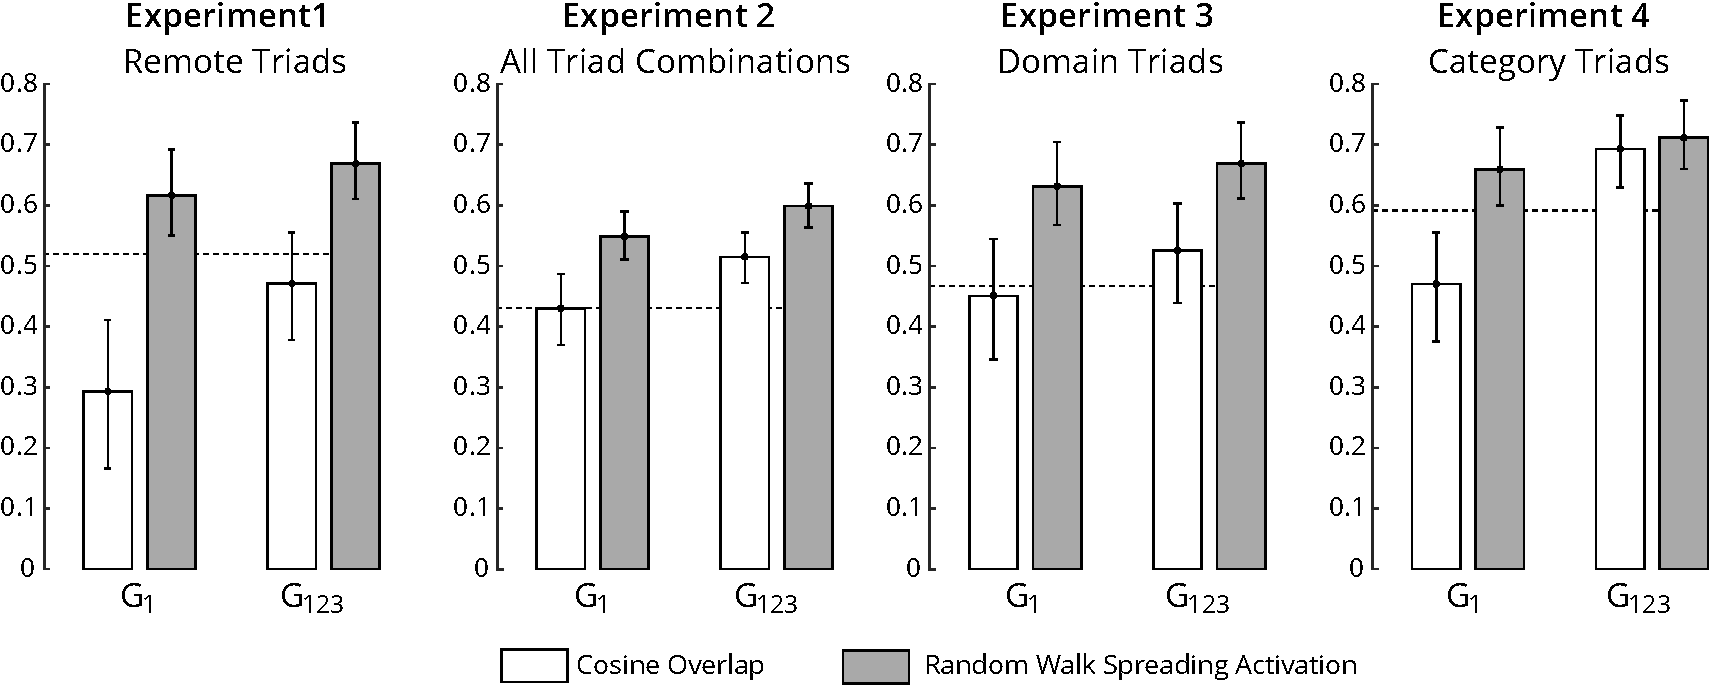
\includegraphics[width=14.5cm]{images/summaryResults6.pdf}
\caption{\small{Correlations and 95\% confidence intervals for the triad preferences and the cosine and random walk model's predictions for all four experiments. As a baseline, the horizontal lines indicate the average person's correlations to the mean population preferences. The random walk spreading activation measure outperforms the cosine measure (except for category-level triads), supporting the idea that the cosine measure accounts for strong but not weak similarity judgments while the random walk measure can account for both. In addition, the denser network ($\mathbf{G}_{123}$) generally outperforms the one constructed from only the first response given by each person ($\mathbf{G}_1$).}}
\label{fig:networkcorrelations}
\end{figure}


The results are shown in Figure~\ref{fig:networkcorrelations}, and a brief inspection reveals the important findings. In almost every case the spreading activation model outperforms the cosine similarity model, and in almost every case the denser graph $\mathbf{G}_{123}$ produces better performance than the sparser graph $\mathbf{G}_1$. To compare the correlations within both types of graphs, $Z$-scores for correlations with a shared third dependent variable \parencite{Steiger1980} were used. For $\mathbf{G}_{1}$, the correlations were significantly higher in all experiments ($Z = -7.51$, $Z = -9.53$, $Z = -4.46$,$Z = -3.88$,  $p < .001$ for each of the four experiments).

For the denser graph $\mathbf{G}_{123}$ the differences were significant for Experiment 1 $Z = -6.46, p < .001$, Experiment 2, $Z = -5.47, p < .001$, Experiment 3, $Z = -5.35, p < .001$ but not for Experiment 4, $Z = -0.03, ns$. The one exception to this pattern is revealing: when modeling the strong similarities collected in Experiment 4 with the richer data set $\mathbf{G}_{123}$, the cosine measure performs comparably to the spreading activation measure. In keeping with our theoretical prediction in the previous section, the value of the semantic network representation is most apparent when considering weaker relationships and weaker connections.


\subsection{The role of activation decay}

The spreading activation model contains a single free parameter $\alpha$, which can be interpreted as a measure of how the spreading activation tends to die away over time. From a modelling perspective, it is important to consider the role that this parameter plays in accommodating the empirical data. The results in Figure~\ref{fig:networkcorrelations} show the performance of the spreading activation model at the best fitting value of $\alpha$. To illustrate how $\alpha$ affects model performance, Figure~\ref{fig:alphaPlot} plots the performance of the spreading activation model for all values of $\alpha$ between 0.1 and 0.95. In general, the model performs better at larger values of $\alpha$, highlighting the fact that the spreading activation model outperforms the cosine model because the former can make good use of more (cfr. the density in Table~\ref{Table:tiger}) and longer associative paths through the semantic network.


\begin{figure}[ht]
\centering
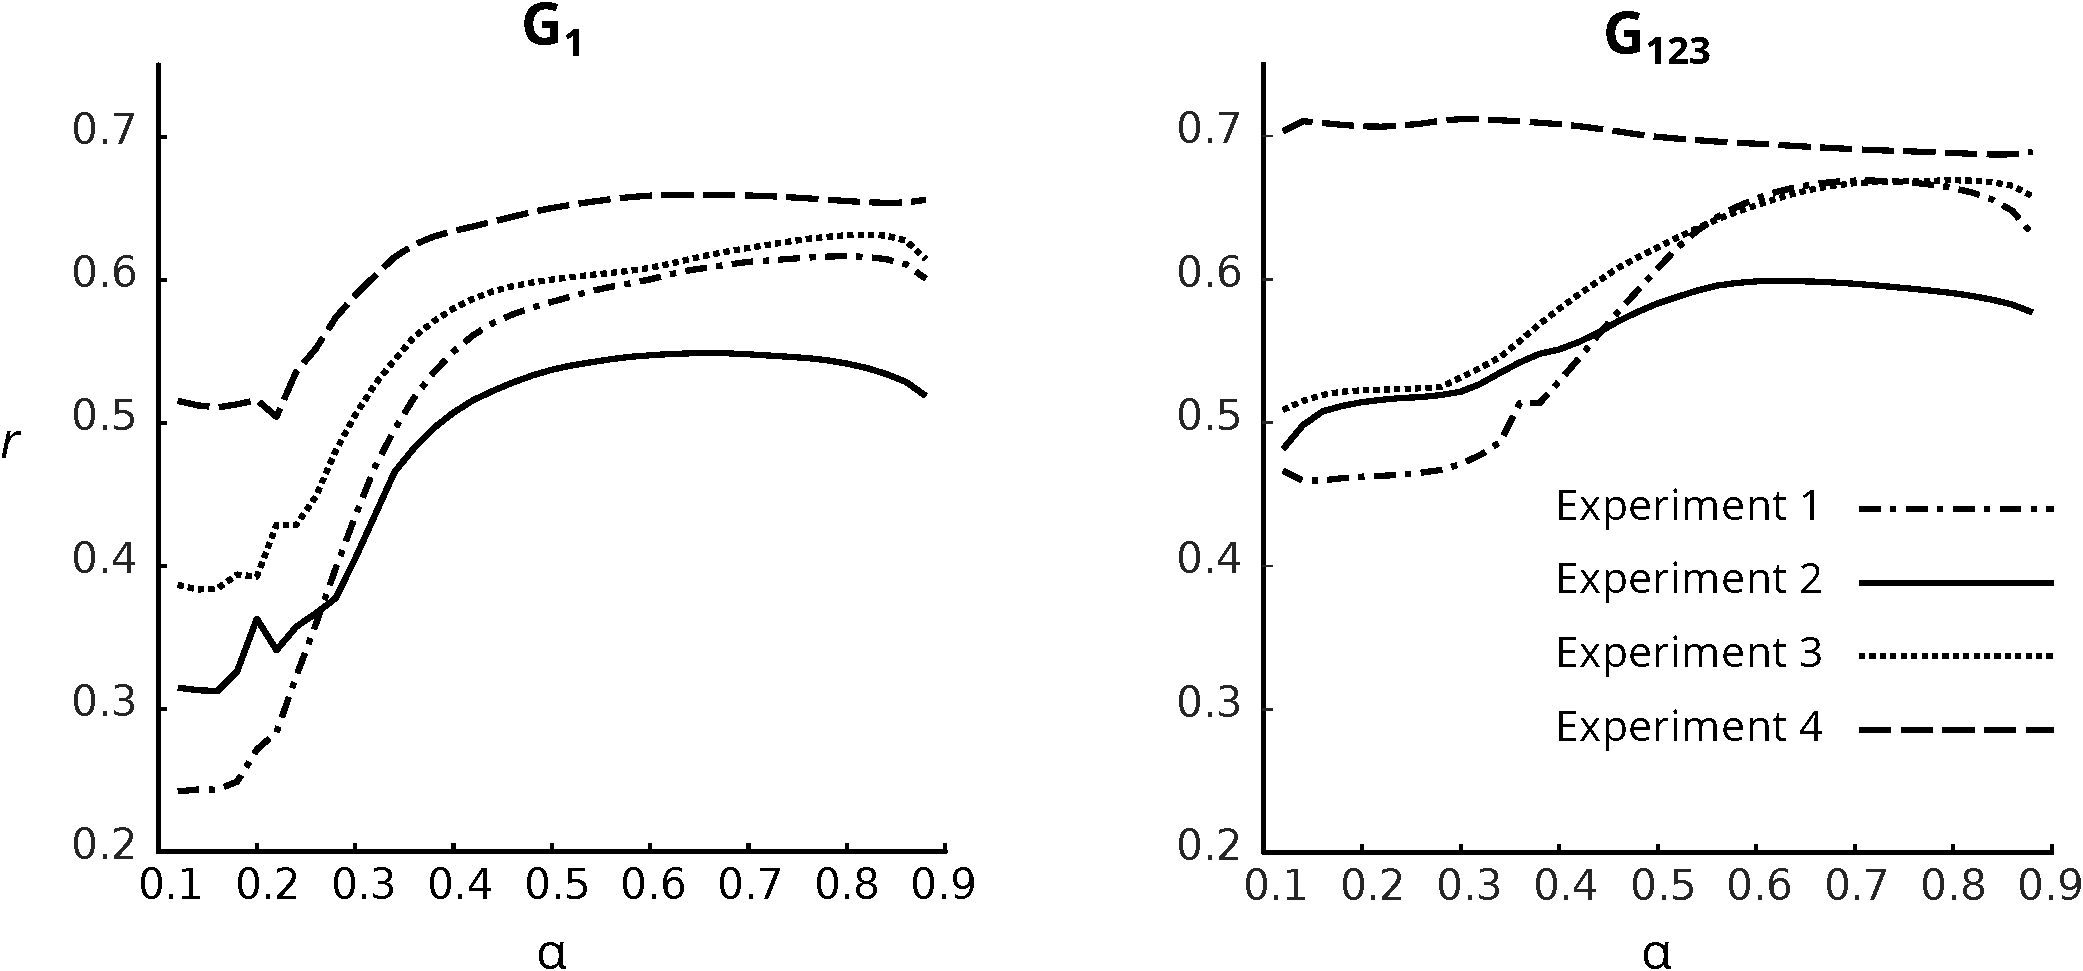
\includegraphics[width=14cm]{images/alphaPlot3.pdf}
\caption{\small{Role of spreading activation parameter $\alpha$ (x-axis) in the prediction of the triadic preferences in four experiments for the single-response graph $\mathbf{G}_{1}$ (left) and the three-response graph $\mathbf{G}_{123}$ (right). The $\alpha$ parameter is a measure of how quickly the spreading activation dies away over time; higher values of $\alpha$ take longer to die away. Overall, performance improves for larger $\alpha$, suggesting that the improved performance of the spreading activation model occurs because it can make good use of longer associative paths through the network.}}
\label{fig:alphaPlot}
\end{figure}




\subsection{Comparing strong and weak similarity using ``small world walks''}
A well documented characteristic of human semantic networks is that they have a small world structure where a network shows a high degree of clustering and at the same time has shorter paths between any pair of nodes  than would be expected given the size of the network \parencite{DeDeyne2008b,Steyvers2005}. In practice, most pairs of concepts can be connected using three or fewer directed links. As a consequence, after just three steps, any node can be activated and additional paths with lengths longer than three (see Equation~\ref{equation_RW_algebraic}) might contribute little information.

A first way to test whether paths of limited length could account for the performance of the random walk is by using the iterative method in Equation \ref{equation_RW_algebraic} for a small number of iterations. Because now the length of the paths is constrained, the frequency bias is less of a concern and the inferred indirect paths would not require an additional weighting step. If indirect paths of length 2 or 3 also aid in the prediction then we would expect that the distributional overlap between two words incorporating indirect paths would improve the prediction over the overlap measure based on direct neighbors.


\begin{figure}[ht]
\centering
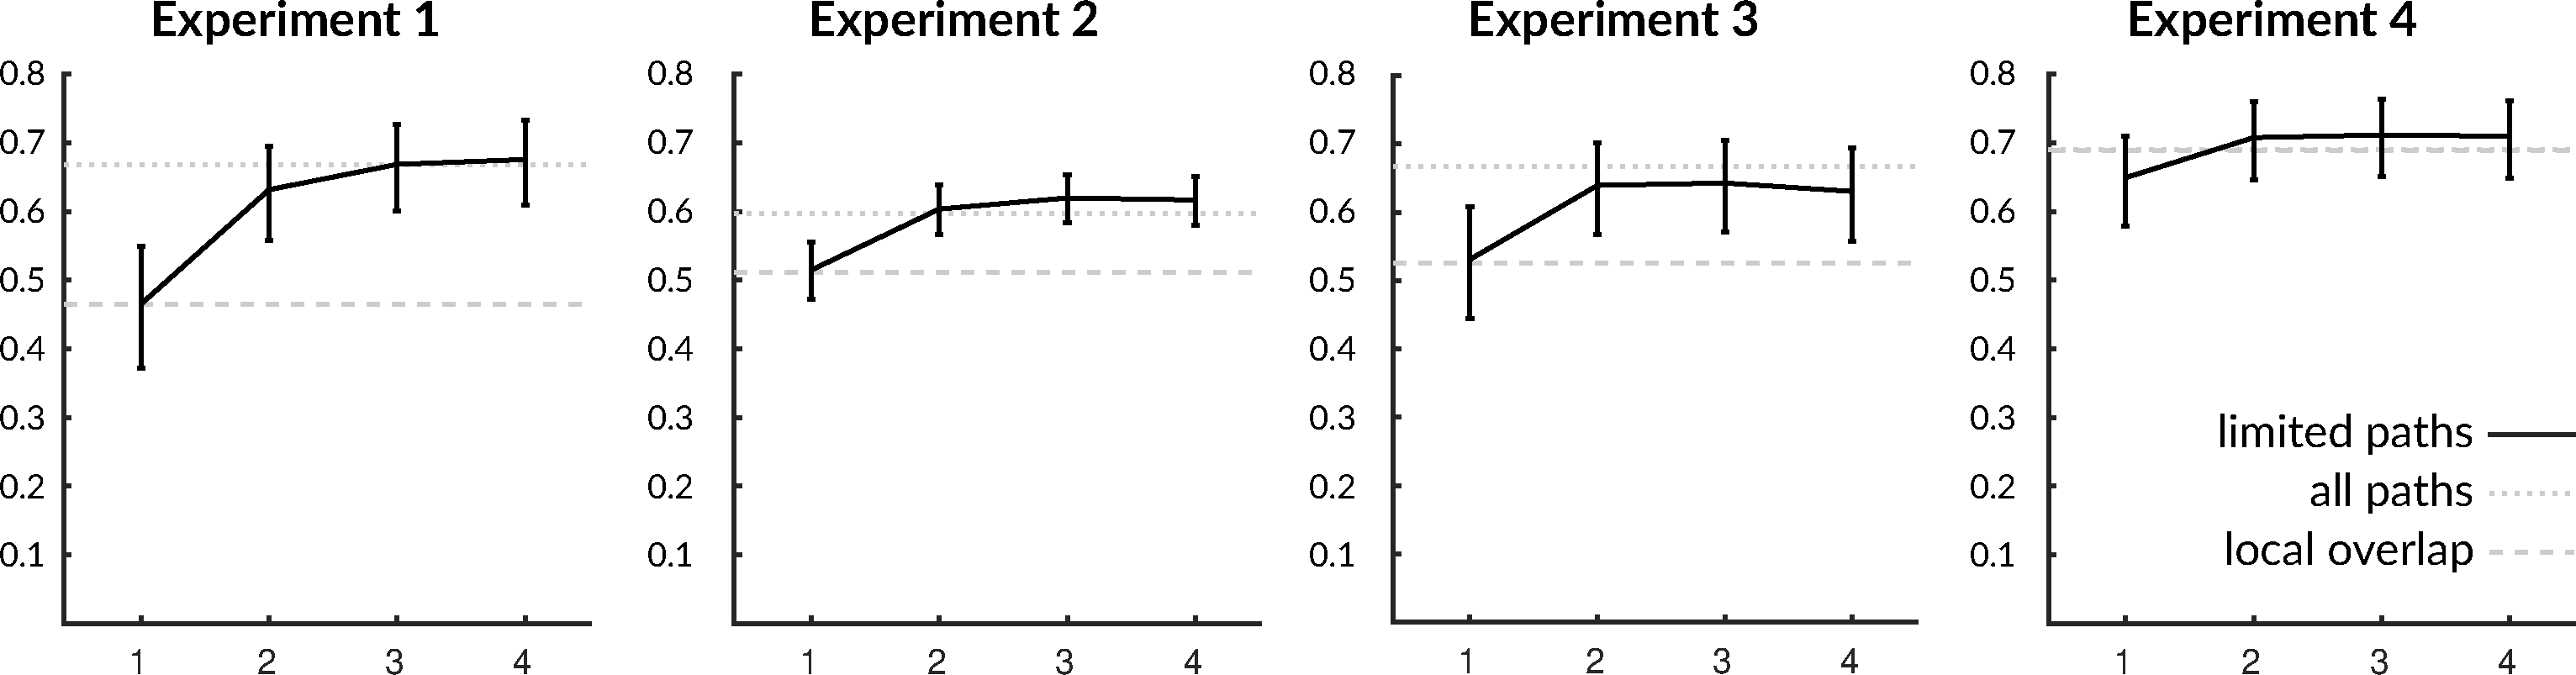
\includegraphics[width=16cm]{images/limitedKatz.pdf}
\caption{\small{Correlations and 95\% confidence intervals for distributional similarity derived on limited walks up to a length of 4 ($x$-axis).}}
\label{fig:limitedWalks}
\end{figure}

The procedure for deriving similarity indices was identical as before and $\alpha$ was again fixed at 0.75.
For the results we will focus on the denser graph $\mathbf{G}_{123}$ as it produces superior results in all experiments so far. The correlations for walks up to a length of 4 are shown in Figure~\ref{fig:limitedWalks}. In each of the experiments we see a considerable improvement by adding indirect paths of length 2, regardless of whether the triads are remote, belong to the same domain or the same category (comparing correlations for paths of length 2 versus length 3 for Experiment 1 to 4: $Z = -6.52$, $Z = -7.40$, $Z = -5.00$, $Z = -5.74$, all $ p < .001$). Adding paths of length 3 somewhat improves the prediction for weak triads in Experiment 1 and 2 (comparing paths of length 3 and 4 were significant only for Experiment 1 and 2: $Z = -5.35$, $Z = -4.37$; all $p < .001$). Paths of length 4 contributed modestly yet significantly in Experiment 1 ($Z = -2.1, p = 0.036$), did not further improve the predictions in Experiments 2 and 4 and adversely affected the prediction in Experiment 3 ($Z = 7.69, p < .001$).
Overall, the results are very similar to the local overlap measure in Figure~\ref{fig:networkcorrelations} and the previous random walk for paths of unbounded length.\footnote{\hspace{0.1cm}Note that the results are quite similar despite the lack of an additional weighting step. This suggests that the additional weighting step is only needed for unbounded walks in Equation \ref{equation_RW_algebraic}.}\footnote{\hspace{0.1cm}The local overlap measure is not entirely identical due to the inclusion of a diagonal term in the first line of Equation \ref{equation_iteration}. The results were very comparable with the largest difference found for Experiment 4, where $r = .65$ for the limited walk versus $r = .68$ for the unbounded walk.}


At this point, we have found indirect similarity by inferring additional links and computing the distributional overlap between the distributions of links of the words in the triads. This provides a good account of the empirical data, whereas the overlap between directly shared features or neighbors can only account for the findings for related triads in Experiment 4.
A second possibility is that the inferred paths themselves could provide us with a way to derive how strongly related the triad pairs are. Such a path-based measure allows us to generalize the paths based on outgoing edges considered in Equation~\ref{equation_RW_algebraic} to incoming edges which might also contribute to predicting remote triads.


\begin{figure}[ht]
\centering
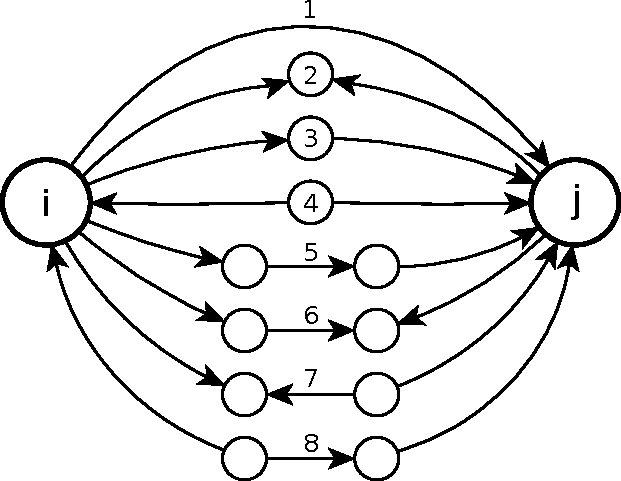
\includegraphics[width=6cm]{images/eightPaths2014.pdf}
\caption{\small{All eight possible paths of length $\leq$ 3 that connect a source node $i$ and target node $j$ in the graph $\mathbf{G}$. Note that because the paths are directed, there are multiple distinct ways to construct paths of the same length (e.g., Paths 2 -- 4 are all of length two).}}
\label{fig:pathIllustration}
\end{figure}

If activation is allowed to flow in both directions, only eight qualitatively distinct ways of connecting two nodes exist for paths of a maximum length of three. These are depicted in Figure~\ref{fig:pathIllustration}. For example, Path 1 corresponds to the situation where there is a direct link between the two nodes (i.e., $i \rightarrow j$), and the probability with which such a path is followed is captured by the transition matrix $\mathbf{P}$ itself. This is the only way in which a path of length one can be formed. In contrast, paths of type 2 and type 3 are the same length, but have a somewhat different interpretation. Path 3 depicts an ``associative chain'' in which a walk starts at node $i$, moves to an intermediate node $k$, and then ends at node $j$ (i.e., $i \rightarrow k \rightarrow j$). The probability associated with any path of this kind can be computed by taking the matrix product $\mathbf{P} \mathbf{P}$. By way of comparison consider path 2, which depicts the ``shared associate'' situation in which nodes $i$ and $j$ both send links to a third node $k$ (i.e., $i \rightarrow k$ and $j \rightarrow k$). The probabilities for paths of type 2 are computed by taking the product $\mathbf{P} \mathbf{P}^T$.


In the original spreading activation model, the various paths are implicitly weighted by their lengths, using a single parameter $\alpha$ to do so. This approach allows no distinction to be made between similarities that people draw on the basis of a ``shared association'' (Path 2) and those formed via ``associative chaining'' (Path 3). A more detailed view of how people assess weak similarities can be obtained if we consider all eight paths separately, and estimate a separate weight $\beta$ for each path type. Formally, this produces the following graph augmented with indirect paths of maximum length $r$ = 3, where  $\sum_i \beta_i = 1$  and  $0 < \beta_i < 1$:


\begin{equation}
\begin{array}{llr}
 \mathbf{G_{r=3}}
  = & \beta_1\mathbf{P} & \text{(paths of length r = 1)}\\
    & + \beta_2\mathbf{P}\mathbf{P}^T + \beta_3\mathbf{P}^2   + \beta_4\mathbf{P}^T\mathbf{P} & \text{(paths of length r = 2)}\\
    & + \beta_5\mathbf{P}^3 + \beta_6\mathbf{P}^2\mathbf{P}^T + \beta_7\mathbf{P}\mathbf{P}^T\mathbf{P} + \beta_8\mathbf{P}^T\mathbf{P}^2  & \text{(paths of length r = 3)}\\
\end{array}
\label{equation_sww}
\end{equation}


This approach unifies overlap measures like the local overlap measure to those taking into account indirect links. In particular, it allows us to compare direct association (Path 1), local overlap (Path 2) with longer paths up to a length of 3.

In line with the spreading activation account, we expect a relatively higher contribution for longer paths in tasks with remote triads in the first three experiment compared to Experiment 4.
To assess whether the indirect paths make a contribution that is statistically reliable, we bootstrapped the path weights in Equation 5 by sampling triads without replacement for 10,000 bootstrap samples. In all four experiments, only a few paths were significant. Across all experiments, there was a consistent contribution of longer paths. As expected we also find a significant contribution for both direct associations and paths of length 2 for the category triads in Experiment 4.
Fitting this more detailed model distinguishing different paths to all four Experiments produces the results depicted in Figure~\ref{fig:pathContributions}.



\begin{figure}[t]
\centering
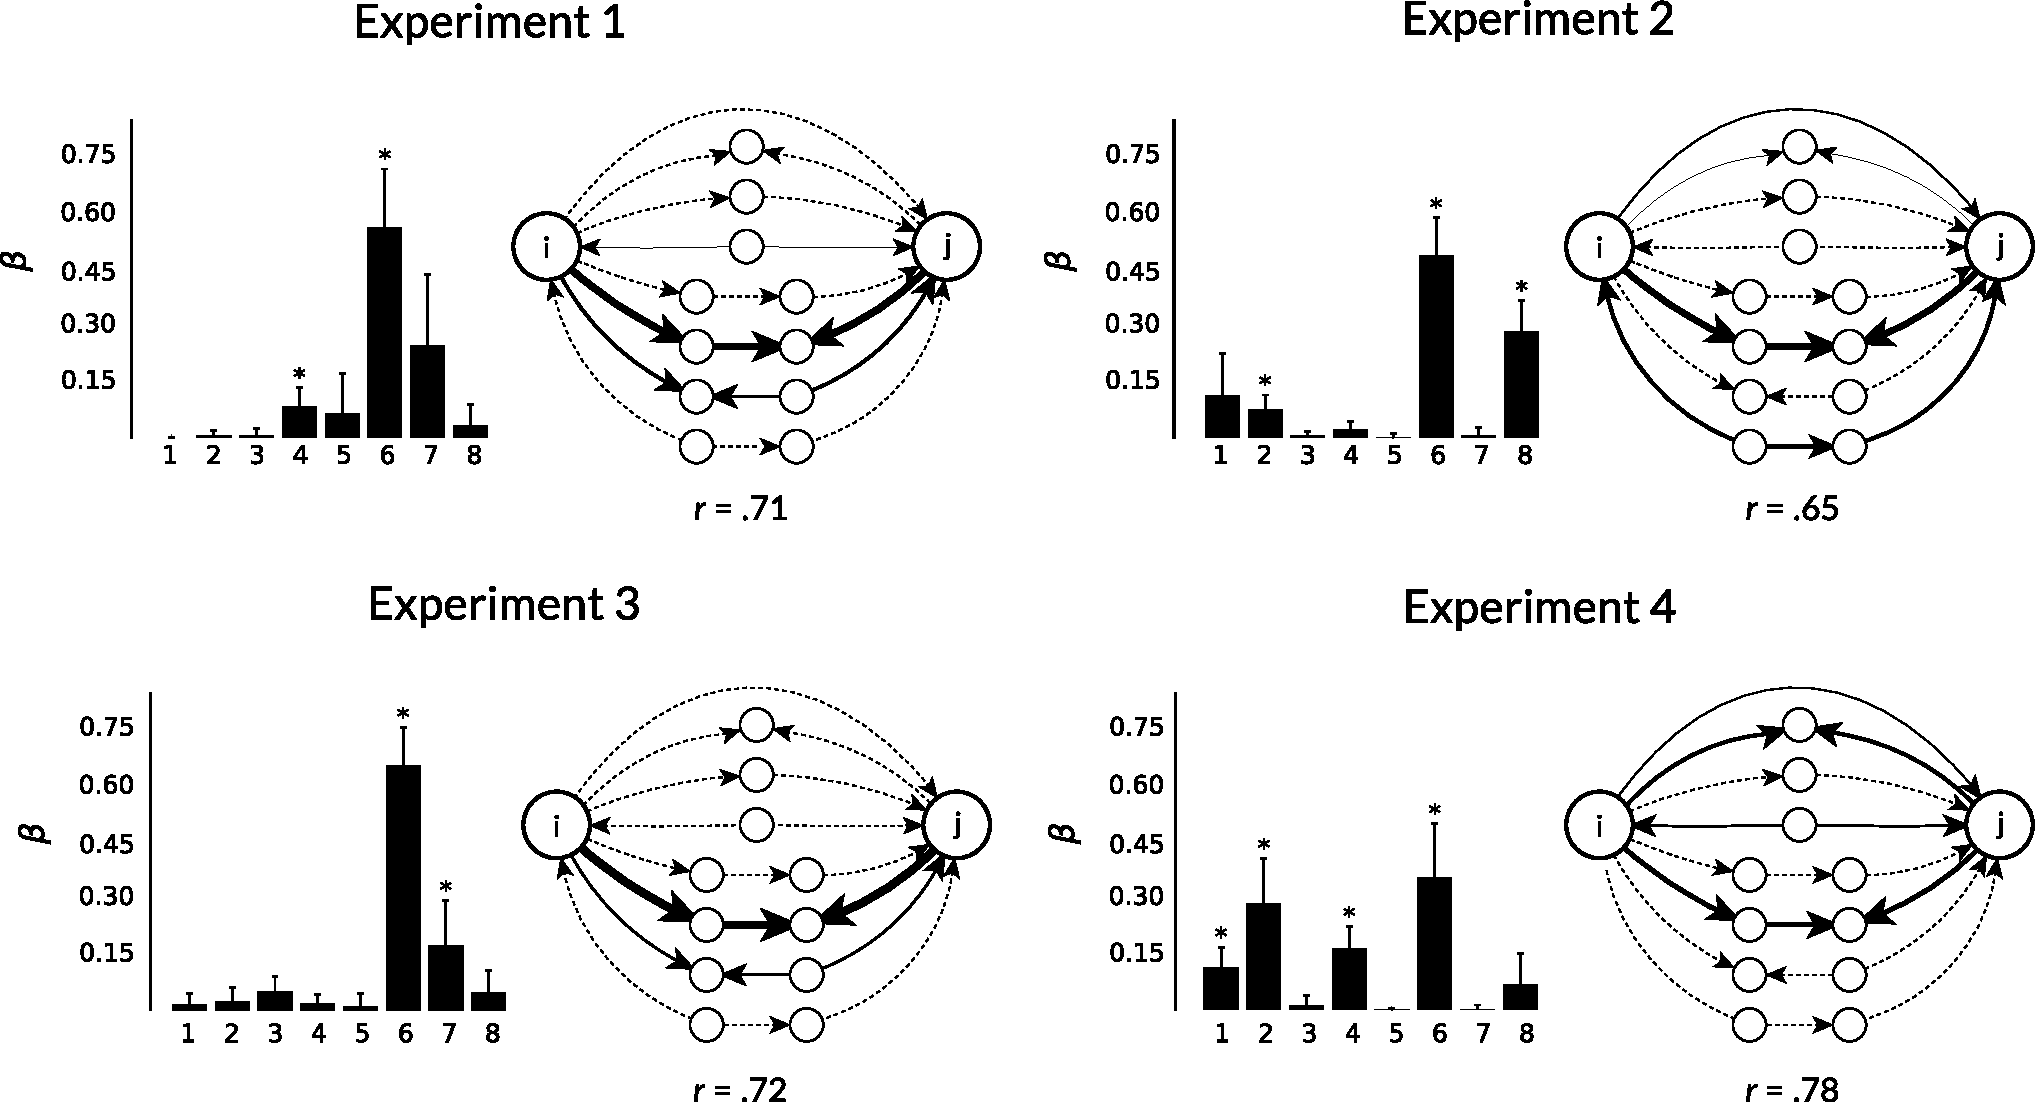
\includegraphics[width=16cm]{images/eightpathsBootstrapped.pdf}
\caption{\small{Path weights for $\mathbf{G}_{123}$ across all four experiments. Numbers on the $x$-axis of the embedded graphs correspond to the path numbers, and the height of the bar graph reflects the weight of that path. The most important paths are indicated by arrows with weights proportional to the thickness of the line. As expected, the longer paths (5--8) make a higher contribution for the tasks with more remote triads (Experiment 1 -- 3). For Experiment 4, which focused on category-level judgments, shorter paths matter relatively more (although the longer paths still play an important role).}}
\label{fig:pathContributions}
\end{figure}




Consistent with our theoretical perspective, we find that the longer paths (i.e., Paths 5--8) are less important in the experiment that relied on strong similarities (Experiment 4) than in the other three experiments, which assessed weaker relationships. Across all experiments we find a particularly strong effect for Path 6 and to a lesser extent Path 2, both of which can be described as a form of ``shared association'' similar to the local distributional overlap discussed previously. This makes sense, given that our experiments presented people with all three items at once. It seems plausible to think that a spreading activation process would be started from all nodes and could ``meet in the middle'' to construct a shared association style connection. In this sense, the contribution of the more direct Path 2 in Experiment 4 also supports the earlier results in which the cosine measure did nearly as well as the random-walk-based measure in that experiment.
Apart from longer paths, this model also allows us to evaluate the contribution of direct associates. This was absent in Experiment 1 by design and in all other experiments except Experiment 4, where it made a modest contribution which isn't surprising for triads like \stimulus{jeans} -- \stimulus{dress} -- \stimulus{skirt} or \stimulus{caterpillar} --  \stimulus{butterfly} -- \stimulus{flea}.

Altogether, we find that a path-based measure performs at least as good or even better as the similarity measure based on indirect paths and in both cases indirect links make a key contribution to the final predictions.

\FloatBarrier

% %%%%%%%%%%%%%%%%%%%%%%%% DISCUSSION %%%%%%%%%%%%%%%%%%%%%%%%

\section{General Discussion}

The main empirical result of this work is that individuals share weak semantic structure, agreeing with each other when making similarity judgments even when those items are apparently unrelated. This supports the idea that the structure tying together remote concepts is shared among individuals. We also demonstrated that it is difficult to reduce the  structure tying together this remote information to simple heuristics like frequency or concreteness matching; it also does not correspond to unidimensional distinctions like whether something is an artifact or animate. Based on an additive tree derived from people's similarity judgments as well as their explicit explanations, we found that people use multiple sources of information when making these judgments, with thematic knowledge playing a key role \parencite[consistent with][]{EstesGolonka2011,Lin2001,Wisniewski1999,Ross1999}.

This pattern of findings was well-explained by a minimalistic spreading activation account based on random walks through a semantic network derived from word-association data. This account captured performance at different levels of the lexicon, from remote associations to domain-level ones to category-level ones. At all of these levels, the spreading activation mechanism allows us to infer information that is not present in the direct connections between a node and its neighbors.

This work also contributes a method for studying the role of indirect paths in semantic networks: examining directed small world walks. This framework includes the commonly used local overlap measure based on shared associates as a special case which can be compared with other types of short directed paths. Similarly, the framework generalizes a commonly used random walk-based global similarity measure to indices of similarity that are not based on ``overlap'' including paths with different directionality. Our results indicate that accessing remote concepts does not necessarily depend on the activation of the entire network \parencite{Ratcliff1994}. Rather, given the small world structure of the network, they can often be accounted for by just a few directed paths with a length of 3 or less.

These results point towards a number of broader theoretical implications. Before getting there, we need to consider other account of relatedness that could explain the systematic preferences in remote triads.

\bigskip

\subsection{Alternative semantic models and the subjective nature of relatedness}



In the introduction we have stressed the notion of relatedness or similarity in the study of concepts and word meaning. Similarity, however, is a property of the perceiver rather than a concept in physical analysis: objects can only be similar or dissimilar to one another in perception (and thought). As argued by Deese and others the notion of similarity is tautological in nature, something is similar when it is similar \parencite[see p 12,][]{Deese1965}. If this is the case, we have to consider where the similarity stems from and render the relation between association and relatedness or similarity more explicit.

In both the current semantic network and other lexico-semantic models derived from text, the links in the network reflects the frequency of occurrence of successive ideas or impressions and ideas in perception and thought. The contiguities that are revealed in the successive instances of thought are those that have occurred frequently enough in the past to have acquired some associative strength \parencite{Deese1965}. According to this associationistic view, relatedness or similarity reflects contiguity by mediation, which allows us to infer that \stimulus{lion} and \stimulus{tiger} are similar because they do not necessary co-occur directly but occur in similar sentences. In other words, they become related in subjective experience. This mental mediation process is similar to the inference in models like LSA \parencite{Landauer1997}, and equally solves the induction problem due to the sparsity in the linguistic environment.
Whereas many lexico-semantic models like LSA stress that the mediated responses are learned rather than dynamically derived using something like spreading activation, the distinction between stored or dynamic representations might be less important than suggested in previous work \parencite{Ratcliff1994,Hare2009} as the mental co-activation of words that never occur together would become stored in memory over time.


All this suggests that other semantic representations or models than the one presented here might equally account for these findings. One possibility is that language models based on information about how words co-occur in the environment should be able to do so too. For such models to infer relationships that never co-occur in text, some kind of abstraction or smoothing over semantic space is needed.  The original LSA model \parencite{Landauer1997}, topic models \parencite{Griffiths2007} and BEAGLE \parencite{Jones2006} all allow for such a mechanism. Because of the availability and abundance of on-line text corpora, reducing sparsity is less of a concern \parencite{Recchia2009}, especially in the case of $n$-gram or co-occurrence models like the Hyperspace Analogue of Language model \parencite{Burgess1998}.

To investigate whether such text-based models could equally account for the preferences in the remote triad task, we ran a pilot study using a Dutch newspaper and online text corpus from which syntactic dependency relations were derived \parencite[see][]{DeDeyne2014CorpusSize}. Although a full treatment of these findings would lead us too far, it is worth mentioning the basic results for comparing the triad judgments across all four experiments. The correlations between the models and people's performance were very similar in all experiments and range from $r = .30$ to $r = .56$. These values are considerably lower compared to those derived from our network model (shown in Figure~\ref{fig:networkcorrelations}). This result is in line with work suggesting that text-based models are less suited to explain human similarity processes because they are based on discourse where communication is the ultimate goal. Compared to word associations, this might provide a very indirect way to access subjective meaning \parencite{Szalay1978,Mollin2009,DeDeyne2014CorpusSize}.

What about linguistically-inspired networks such as WordNet? They might account for people's shared weak similarity judgments, since they represent a fully connected hierarchical network with a large variety of words. Moreover, they allow an interesting test case as the relations are primarily defined by category-based similarity. To investigate to what degree this kind of hierarchical semantic representation can capture our findings we derived relatedness measures from Cornetto \parencite{Vossen2013}, which expands previous versions of the Dutch version of WordNet. This semantic network consists of 92,000 lemmas for which 118,000 word meanings are encoded. Using the best performing path-based similarity measure, we found no significant correlation between network predictions and people's performance in Experiment 1 and weak correlations in Experiment 2 and 3 ($r = .17, p < .01$ and $r = .14, p < .01$). The results were better at the level of basic level categories (Experiment 4, $r = .26, p < .01$), but still not close to the findings based on the cosine or spreading activation indices derived from the word association network. This suggests that a very extensive linguistic expert system like WordNet does not capture the mental properties underlying the relationships between remote concepts.

Perhaps the importance of other kinds of information is not accounted for in a way that corresponds with how humans mentally represent concepts.
Alternatively, this could be due to the fact that the crucial (thematic) information is missing.
Due to the distributional properties of language, a word can only be related to a small number of other words but can systematically co-occur with a much larger set of words. As a consequence, the fundamental relation in lexico-semantic models is of a thematic nature, defined in a broad sense as two entities that co-occur in a temporal or spatial context.


 Furthermore, a study on the taxonomic category structure of the same association-based semantic network found a systematic thematic structure at each level of the taxonomy \parencite{DeDeyneVerheyenNavarro2015}.
 While this suggested a different organization compared to similarity-based taxonomic models like WordNet, one might object that this simply reflects the procedure of collecting word associations. However, this study demonstrated that restricting the range of concepts to concrete nouns like the one studied in Experiment 4 was able to recover a taxonomy grouping well-known categories like \stimulus{birds} or \stimulus{tools}. This suggests that similarity-based taxonomies arise from a selection bias for concrete nouns belonging to a relative small set of categories.

Finally, one might argue that this reflects the specific triadic comparisons used in this study as well. However, the pattern of results observed here for both WordNet and text corpus based models has also been observed on related tasks such as human similarity ratings; these models only accounted for a portion of the variance captured by network models derived from word associations \parencite{DeDeyne2009,DeDeyne2014CorpusSize}.


\subsection{Factors affecting model performance}


We identified four factors that determine the prediction performance of our semantic network model. A first one is the type of comparison: the best performance was found for the more closely related triads (in which the items all came from the same category), although performance was still high for the more remote ones. A second factor is the density of the graph: as earlier work demonstrated, denser graphs led to better predictions \parencite{DeDeyne2013b}. The role of information spreading was also proportionally larger in very sparse graphs ($\mathbf{G}_1$), which might indicate potential ceiling effects in very dense graphs. This was supported by the finding for the categoric triads and the denser graph $\mathbf{G_{123}}$, which were nearly identical for the local overlap and spreading activation measures. A third factor is the decay parameter $\alpha$, which confirmed that tasks with more remote triads benefit from longer indirect paths. Closely related to the decay factor we also confirmed that length of the path itself played a similar role. This was both apparent in small world walks over undirected paths up to a length of 4, and a more general approach that also includes directed paths up to a length of three. While both analyses derive similarity in a slightly different way, they both showed a contribution of longer paths, especially in those experiments with remote triads.

\bigskip



\subsection{Implications for theories about semantic representations}

One of the main implications of our work is that information about remote concepts is represented in a stable way. This is interesting in light of the logical problem of similarity construction discussed in the introduction. One possibility is that the nature of the structure underlying remote concepts is constrained by limitations in how humans perceive the world and process input. These constraints might exert a strong top-down influence in detecting structure, even if such structure is absent in the environment. While such constraints must certainly exist to some extent, it is unclear whether they are sufficient to explain how or why people have such similar judgments about very weakly-related concepts.

Another possibility is that the way the environment (linguistic or otherwise) is structured represents a form of learning that contributes strongly to the structure of our mental representations. For instance, consider the emphasis our participants placed on thematic knowledge. This sort of knowledge is acquired naturally from language \parencite{EstesGolonka2011} as well as contingencies in the environment. Thematic information plays such a strong role that it has even been found to override taxonomic judgments \parencite{Lin2001,Wisniewski1999}. People's ability to detect and use weak correlations in language and the environment is also apparent in the existence of spurious correlations in synaesthesia as well as the phenomenon of \textit{pareidolia} where the mind perceives patterns where none actually exist in the patterns of clouds, rocks or even coffee foam \parencite[e.g.,][]{Liu2014}.

Schizophrenia is another case where people may impose structure on weakly-related items. In that case, disturbed language production has been characterized as the loosening of associations, the intrusion of mediated responses and the presence of hyper-priming due to a presumed lack of ability to inhibit weak links \parencite{Pomarol-Clotet2008}. In this case, the seemingly bizarre pathological responses  produced in a word association task may have a sensible explanation based on relationships between distant items in a semantic network \parencite{Gordon1982}. Altogether, these phenomena suggest that at least to some extent, people impose or infer some structure when organizing their semantic knowledge, and they do so in similar ways to each other. The most interesting question for cognitive scientists is what imposes those constraints, how that structure is organized, and how that affects the way in which we process information.

Our experiments suggest some answers to these questions. In Experiment 2, we found that no single factor (like a domain or a feature) accounted for people's similarity judgments, even though that information was available. The introspective judgments in Experiment 3 indicated that most participants related pairs through a thematic link; this aligns with previous results that showed that the dominant type of information represented in semantic networks from word associations is thematic \parencite{DeDeyne2008b}. If this is indeed the case, then the notion of what constitutes a natural category \parencite[e.g., as proposed by][ as an organizing factor of the mental lexicon]{Rosch1973} based on entity features needs to be expanded. Our findings contribute to a larger body of research suggesting that even the taxonomic structure in the animal domain needs to be questioned because such a taxonomic organization of knowledge might be heavily culturally defined \parencite{LopezAtran1997} or a consequence of formal education \parencite{SharpCole1979}.

Similarly, due to the free nature of the association task (in contrast to the property generation task), the semantic network cannot be described as encoding a single type of information as it captures both thematic and featural relations under the form of temporal contiguities (\stimulus{jungle} -- \stimulus{tiger}) and similarity relations (\stimulus{lion} -- \stimulus{tiger}).

A final contribution of this research is that it can account for asymmetry effects in various tasks including similarity judgments \parencite[e.g.,][]{Tversky1977}. Representing the mental lexicon as a directed graph explicitly incorporates the idea of asymmetry. Indeed, our modelling work indicates that the direction of the links and paths connecting any pair of words influences the retrieval of information significantly. This suggests that while previous work has often transformed representations to undirected networks for reasons of simplicity \parencite[e.g.,][]{Steyvers2004}, the availability of sophisticated graph-theoretic measures for directed networks is a viable alternative and may be more appropriate in some cases.

Our explicit account for how information spreads over short directed paths also has implications for priming research. First, asymmetry effects for associative priming has been used to distinguish it from pure semantic priming \parencite{Thompson-Schill1998}. Our results indicate that these distinctions can be refined further by not only considering directly associated prime and target pairs, but by also looking at indirect directed paths that could give rise to asymmetry as well.
Second, the small world walks also provide a well defined framework to study mediated priming, which has been of theoretical significance for the study of activation spreading \parencite{Hutchison2003}. In this priming task facilitation for a target word such as \stimulus{lion} is observed after primes like \stimulus{stripes} even though both words are not directly related. Instead activation spreads through an intermediate node, in this case \stimulus{tiger}. This example corresponds to one of the potential paths connecting prime and target, whereas potential other directed paths (see Figure~\ref{fig:pathIllustration}) or a combination of them might be able to provide a more systematic framework to test semantic processing in priming.

\bigskip

\subsection{Open questions and future directions}
The stability of weak semantic structure, ways of assessing this empirically, and initial steps to predict this behavior are in many ways just the beginning of a new chapter which has the potential to bring together different research areas.
Specifically, it highlights specific predictions that can only be answered partially based on the current data.

A first question is how a computational model might account for the decision latencies in the remote triad task. Starting with the \textcite{Collins1975} network models, one expects spreading activation on longer paths leading to slower RTs. Although an RT analysis was not the main purpose of this study, we did find that those triads participants responded to faster had paths that were somewhat shorter than harder triads with long reaction times (especially in Experiment 4). Similarly, for triads in which people responded quickly, the model performs well, with correlations between 0.68 and 0.87. It performs somewhat less well on the slower trials (which presumably correspond to the more difficult decisions), although even there the correlations are still respectable, ranging between 0.53 and 0.66.
Of course modeling reaction times in triadic decision tasks presents additional challenges as well, like response competition and so on, whereas our models of spreading activation and the integration of information in the remote triad task were chosen with transparency and interpretability in mind and were therefore fairly simple.

While the interpretation of the present results on RTs is highly speculative, they do indicate this might be an interesting avenue for future research. One way would be by incorporating more information about the timing aspects of the decision process. Recent mathematical models for reaction times might allow us to get a better understanding of how the choices are made based on the accumulation of evidence for each pair in the triad. These models include drift-diffusion \parencite{Ratcliff1978} or linear ballistic models \parencite{BrownHeathcote2008}. Another approach would involve unraveling the information processing constraints in terms of  parallel, serial or coactivated processing \parencite{TownsendNozawa1995}.

If the mental lexicon is not structured primarily as a similarity-based hierarchical taxonomy but reflects a more thematic-based organization, one might also question what type of similarity process determines how we retrieve this primarily thematic information from the mental lexicon.
For highly similar entities such as \stimulus{lions} and \stimulus{tigers} similarity might depend on the alignability of the entity properties shared by visual similar entities \parencite{Markman1993}. This contrasts with another possibility that does not rely on intrinsic feature overlap but relies on a process of thematic integration when no intrinsic features match \parencite{WiemerHastingsXu2003,Wisniewski1999,Lin2001}.  On the basis of previous research two distinct predictions can be made. On the one hand, similarity between verbs or abstract nouns primarily depends on a process of thematic integration \parencite{WiemerHastingsXu2003} which suggests that all things being equal, different types of comparison processes might determine triadic preferences depending on the type of word.
Second, in the case of concrete concepts, one might suspect the alignment of common features to be situated at the basic level as this level encodes similar shape and function \parencite{Rosch1976a} whereas integration might be more natural when such aligneable features are not present.
While this prediction is largely supported by the current results through the contribution of different types of paths depending on the range of concepts (weakly related nouns in Experiment 1 vs nouns from a common category in Experiment 4), it remains to be seen if the same hold for other concepts than concrete nouns that might be varied in terms of their taxonomic relation.


A final prediction that follows from the associationist account where weak linguistic contingencies are encoded is that the weak similarity structure might change in a continuous fashion from childhood to late language development. If language exposure automatically leads to the activation of mediated representations, additional exposure should change the way we structure the mental lexicon. This type of representational change has been documented in the case of the syntagmatic-to-paradigmatic shift in children \parencite{Ervin1961} and an ongoing large-scale cross-sectional study in our lab suggests this qualitative shift unfolds continuously throughout adulthood.
 The semantic network provides a static snapshot of this proces as it contains an increasing amount of higher-order associations with time whereas the spreading activation mechanism illustrates how these higher-order links might be gradually learned as a function of language exposure.

Overall, although much work remains to be done, this research suggests that expanding the area of study by including weak similarities can be a significant step forward to differentiate different theoretical proposals and more generally understanding both the nature of people's semantic networks and how information is accessed within them.

\printbibliography

\newpage
\begingroup
\parindent 0pt
\parskip 2ex
\def\enotesize{\normalsize}
\theendnotes
\endgroup

% Note the smash command to make sure the underlining ison the same level (pjg vs wrt)
\begin{appendix}
\section{Remote triad stimuli used in Experiment 1}
\begin{small}
The triads are ordered from weak preferences to strong preferences, with the modal response indicated by
boldface words. In the case of ties, the second pair is underlined.


\begin{longtable}{ll}
\label{table:AppendixRemoteTriads}
Stimulus  & English Translation\\
\toprule
\endfirsthead

Stimulus  & English Translation\\
\toprule
\endhead

\bottomrule
\multicolumn{2}{r}{Continued on next page} \\
\endfoot

\bottomrule
\endlastfoot
\textbf{haat} -- ochtend -- \textbf{toets} & hate -- morning -- test\\
\textbf{bandiet} -- \underline{\smash{bes}} -- \underline{\smash{\textbf{fanfare}}} & bandit -- berry -- fanfare\\
\textbf{gorilla} -- riet -- \textbf{rover} & gorilla -- reed -- robber\\
\textbf{beer} -- engel -- \textbf{hoed} & bear -- angel -- hat\\
\textbf{duister} -- hitte -- \textbf{schot} & darkness -- heat -- shot\\
\textbf{kanarie} -- \textbf{pion} -- vuilnis & canary -- pawn -- garbage\\
\textbf{banaan} -- \textbf{fee} -- onweer & banana -- fairy -- storm\\
bluts -- \textbf{buidel} -- \textbf{veter} & bump -- pouch -- shoestring\\
\textbf{bokaal} -- \textbf{korrel} -- magneet & jar -- kernel -- magnet\\
\textbf{pret} -- taart -- \textbf{zang} & fun -- pie -- singing\\
speld -- \textbf{tegel} -- \textbf{troon} & pin -- tile -- throne\\
\textbf{eind} -- \textbf{risico} -- vaart & end -- risk -- canal\\
\textbf{duikboot} -- \underline{\smash{\textbf{poef}}} -- \underline{\smash{vlaai}} & submarine -- pouf -- flan\\
\textbf{alarm} -- \textbf{kreng} -- orgel & alarm -- carrion -- organ\\
anker -- \textbf{kramp} -- \textbf{slip} & anchor -- cramp -- briefs\\
\textbf{bijbel} -- leeuw -- \textbf{vlot} & Bible -- lion -- raft\\
donder -- \textbf{spuug} -- \textbf{ton} & thunder -- spittle -- ton\\
doos -- \textbf{schat} -- \textbf{sleutel} & box -- treasure -- key\\
\textbf{atleet} -- knuppel -- \textbf{koord} & athlete -- bat -- cord\\
\underline{\smash{\textbf{barbecue}}} -- \textbf{cassette} -- \underline{\smash{mest}} & barbecue -- cassette -- manure\\
\textbf{dienaar} -- \textbf{kier} -- meel & servant -- crack -- plain flour\\
\textbf{dam} -- \textbf{rups} -- tang & dam -- caterpillar -- pliers\\
koor -- \textbf{sap} -- \textbf{spade} & choir -- juice -- spade\\
\textbf{haan} -- rok -- \textbf{sneeuw} & rooster -- skirt -- snow\\
\textbf{kroon} -- \textbf{reus} -- toeter & crown -- giant -- horn\\
kabel -- \textbf{kruid} -- \textbf{prop} & cable -- weed -- gag\\
idioot -- \textbf{vitamine} -- \textbf{zondag} & idiot -- vitamin -- Sunday\\
\textbf{pastoor} -- \textbf{vleugel} -- voetbal & pastor -- wing -- soccer ball\\
\textbf{actie} -- klant -- \textbf{slag} & action -- customer -- stroke\\
\textbf{beroep} -- \textbf{gevaar} -- rust & profession -- danger -- half time\\
\textbf{afdak} -- beschuit -- \textbf{elastiek} & overhang -- rusk -- elastic\\
\textbf{paling} -- \textbf{stengel} -- tunnel & eel -- stem -- tunnel\\
\textbf{bom} -- gips -- \textbf{haard} & bomb -- plaster cast -- fireplace\\
\textbf{beker} -- hagel -- \textbf{juf} & cup -- hail -- teacher\\
korst -- \textbf{schrift} -- \textbf{vlinder} & crust -- writing -- butterfly\\
\textbf{akker} -- \textbf{deeg} -- knuffel & field -- dough -- stuffed animal\\
\textbf{horloge} -- koningin -- \textbf{vierkant} & watch -- queen -- square\\
\textbf{gewicht} -- lawaai -- \textbf{oefening} & weight -- noise -- exercise\\
\textbf{koffer} -- \textbf{mes} -- plein & suitcase -- knife -- square\\
\textbf{kwartier} -- \textbf{proef} -- voertuig & quarter -- test -- vehicle\\
\textbf{hyena} -- radijs -- \textbf{salto} & hyena -- radish -- somersault\\
\textbf{biscuit} -- bokser -- \textbf{poedel} & biscuit -- boxer -- poodle\\
kreeft -- \textbf{postbode} -- \textbf{splinter} & lobster -- mail carrier -- splinter\\
\textbf{gids} -- kalk -- \textbf{pupil} & guide -- chalk -- pupil\\
\textbf{fles} -- hok -- \textbf{vent} & bottle -- hutch -- guy\\
\textbf{klem} -- \textbf{storm} -- vrucht & clamp -- storm -- fruit\\
borstel -- \textbf{poep} -- \textbf{worm} & brush -- buttocks -- worm\\
hengel -- \textbf{mais} -- \textbf{tros} & fishing rod -- corn -- bunch\\
\textbf{diefstal} -- \textbf{som} -- vouw & theft -- sum -- fold\\
\textbf{boel} -- gebed -- \textbf{gek} & lot -- prayer -- crazy\\
hal -- \textbf{ramp} -- \textbf{ruiter} & hall -- disaster -- rider\\
rijm -- \textbf{tocht} -- \textbf{vrede} & rhyme -- tour -- peace\\
\textbf{agent} -- mouw -- \textbf{prins} & cop -- sleeve -- prince\\
\textbf{arend} -- \textbf{plons} -- robot & eagle -- splash -- robot\\
hooi -- \textbf{kraal} -- \textbf{sultan} & hay -- bead -- sultan\\
\textbf{paprika} -- rubber -- \textbf{zwaluw} & bell pepper -- rubber -- swallow\\
\textbf{eekhoorn} -- spar -- \textbf{valk} & squirrel -- fir -- falcon\\
\textbf{boete} -- dooi -- \textbf{hostie} & penalty -- thaw -- wafer\\
\textbf{oma} -- \textbf{suiker} -- wortel & grandmother -- sugar -- root\\
adem -- \textbf{gezin} -- \textbf{hotel} & breath -- family -- hotel\\
\textbf{bretel} -- dweil -- \textbf{lasso} & suspender -- floorcloth -- lasso\\
\textbf{cement} -- \textbf{oprit} -- riool & cement -- driveway -- sewer\\
\textbf{abdij} -- \textbf{inbraak} -- prul & abbey -- burglary -- bauble\\
\textbf{driehoek} -- \textbf{lade} -- tijger & triangle -- drawer -- tiger\\
\textbf{meeuw} -- \textbf{mos} -- trompet & gull -- moss -- trumpet\\
\textbf{doorn} -- parel -- \textbf{pleister} & thorn -- pearl -- bandage\\
\textbf{balkon} -- \textbf{blok} -- klauw & balcony -- block -- claw\\
\textbf{heks} -- kraan -- \textbf{vet} & witch -- crane -- fat\\
\textbf{taak} -- verte -- \textbf{zonde} & task -- distance -- sin\\
\textbf{haag} -- navel -- \textbf{pauw} & hedge -- belly button -- peacock\\
abrikoos -- \textbf{bever} -- \textbf{ekster} & apricot -- beaver -- magpie\\
panter -- \textbf{spaak} -- \textbf{tube} & panther -- spoke -- tube\\
\textbf{bijl} -- \textbf{twijg} -- wijf & ax -- twig -- woman\\
\textbf{boerin} -- duin -- \textbf{gebit} & peasant woman -- dune -- teeth\\
\textbf{kilo} -- melodie -- \textbf{stank} & kilo -- melody -- stench\\
\textbf{cake} -- pijp -- \textbf{snee} & cake -- pipe -- slice\\
kolom -- \textbf{ober} -- \textbf{zuur} & column -- waiter -- acid\\
\textbf{duivel} -- meid -- \textbf{pater} & devil -- maid -- father\\
\textbf{douche} -- \textbf{luier} -- tekening & shower -- diaper -- drawing\\
\textbf{lezer} -- \textbf{priester} -- wijk & reader -- priest -- district\\
\textbf{kameel} -- \textbf{luipaard} -- specht & camel -- leopard -- woodpecker\\
\textbf{camping} -- \textbf{eik} -- zweep & camping -- oak tree -- whip\\
boter -- \textbf{trein} -- \textbf{zadel} & butter -- train -- saddle\\
\textbf{berg} -- \textbf{eiland} -- kring & mountain -- island -- circle\\
\textbf{libel} -- \textbf{raaf} -- spons & dragonfly -- raven -- sponge\\
\textbf{diarree} -- jurk -- \textbf{soep} & diarrhea -- dress -- soup\\
\textbf{boon} -- pijl -- \textbf{snoep} & bean -- arrow -- candy\\
\textbf{bioscoop} -- \textbf{camera} -- damp & cinema -- camera -- vapor\\
\textbf{draad} -- \textbf{pet} -- tomaat & thread -- cap -- tomato\\
datum -- \textbf{gif} -- \textbf{lek} & date -- poison -- leak\\
\textbf{leerling} -- \textbf{maat} -- nest & student -- measure -- nest\\
\textbf{gieter} -- inktvis -- \textbf{theepot} & watering can -- squid -- teapot\\
\textbf{herrie} -- \textbf{stoet} -- zwam & racket -- parade -- fungus\\
\textbf{bestek} -- \textbf{dessert} -- tractor & cutlery -- dessert -- tractor\\
\textbf{goudvis} -- handtas -- \textbf{parkiet} & goldfish -- handbag -- parakeet\\
\textbf{havik} -- \textbf{pelikaan} -- vloed & hawk -- pelican -- flood\\
\textbf{krokodil} -- \textbf{papegaai} -- vlek & crocodile -- parrot -- stain\\
\textbf{merel} -- \textbf{pony} -- servet & blackbird -- pony -- napkin\\
\textbf{beha} -- ijskast -- \textbf{sport} & bra -- refrigerator -- sport\\
asiel -- \textbf{braam} -- \textbf{gelei} & asylum -- blackberry -- jelly\\
\end{longtable}
\end{small}


\section{Stimuli Experiment 2}

\begin{small}
\begin{longtable}{llll}
\label{table:AppendixBIBD}
Stimulus  & English Translation & Valence & Imageability\\
\toprule
adem & breath & 4.78 & 5.63 \\
akker & field & 4.29 & 6.13\\
asiel & asylum & 2.83 & 5.40\\
atleet & athlete & 5.03 & 6.23\\
berg & mountain & 4.45 & 6.72\\
bom & bomb & 2.08 & 6.47\\
boter & butter & 4.09 & 6.40\\
donder & thunder & 3.11 & 4.98\\
kameel & camel & 4.39 & 6.07\\
koord & cord & 4.03 & 6.00\\
korrel & grain & 4.00 & 5.27\\
korst & crust & 3.58 & 5.80\\
kraan & crane & 4.11 & 6.63\\
kring & circle & 4.48 & 5.90\\
melodie & melody & 5.39 & 4.20\\
orgel & organ & 4.23 & 5.52\\
paling & eel & 3.70 & 5.71\\
poedel & poodle & 3.92 & 6.30\\
priester & priest & 3.52 & 5.85\\
sleutel & key & 4.44 & 6.43\\
taak & task & 3.77 & 3.43\\
tijger & tiger & 4.48 & 6.20\\
vuilnis & garbage & 2.64 & 6.53\\
worm & worm & 3.17 & 5.87\\
zwaluw & swallow & 4.55 & 6.00\\
\bottomrule
\end{longtable}
\end{small}



\section{Stimuli Experiment 3}
\label{Appendix:DomainTriads}

\begin{small}
\begin{longtable}{lll}
\caption[Artifact Domain Triads in Experiment 3.]{Artifact Domain Triads in Experiment 3.}\\
\label{table:AppendixArtifactsDomain}

Stimulus & English Translation & Category \\
\toprule
\endfirsthead

Stimulus & English Translation & Category \\
\toprule
\endhead

\bottomrule
\multicolumn{3}{r}{Continued on next page} \\
\endfoot

\bottomrule
\endlastfoot

bloes--handdoek--zeppelin & blouse--towel--Zeppelin & clothing--kitchen utens.--vehicles \\
beha--frigo--viool & bra--fridge--violin & clothing--kitchen utens.--music instr. \\
jas--microgolf--saxofoon & coat--microwave oven--saxophone & clothing--kitchen utens.--music instr. \\
jogging--triangel--zwaard & tracksuit--triangle--sword & clothing--music instr.--weapons \\
kleed--ploeg--zeef & dress--plough--sieve & clothing--tools--kitchen utens. \\
sweater--vijl--weegschaal & sweater--file--scales & clothing--tools--kitchen utens. \\
hemd--raket--tank & shirt--rocket--tank & clothing--vehicles--weapons \\
broek--speer--wok & pants--spear--wok & clothing--weapons--kitchen utens. \\
fles--jeans--tractor & bottle--jeans--tractor & kitchen utens.--clothing--vehicles \\
mixer--pyjama--vliegtuig & mixer--pyjamas--airplane & kitchen utens.--clothing--vehicles \\
fornuis--hoed--moto & stove--hat--motorbike & kitchen utens.--clothing--vehicles \\
pan--tamboerijn--tram & pan--tambourine--tram & kitchen utens.--music instr.--vehicles \\
koffiezet--waterpas--zweep & percolator--level--whip & kitchen utens.--tools--weapons \\
blikopener--bus--harp & can opener--bus--harp & kitchen utens.--vehicles--music instr. \\
klopper--touw--trein & whisk--rope--train & kitchen utens.--weapons--vehicles \\
klarinet--topje--zaag & clarinet--top--saw & music instr.--clothing--tools \\
piano--riem--slede & piano--belt--sled & music instr.--clothing--vehicles \\
panfluit--rasp--stok & pan flute--grater--stick & music instr.--kitchen utens.--weapons \\
gitaar--lepel--zwempak & guitar--spoon--bathing suit & music instr.--kitchen utens.--clothing \\
doedelzak--schop--theelepel & bagpipe--shovel--teaspoon & music instr.--tools--kitchen utens. \\
drumstel--koets--vork & drum set--carriage--fork & music instr.--vehicles--kitchen utens. \\
banjo--dolk--kom & banjo--dagger--bowl & music instr.--weapons--kitchen utens. \\
accordeon--katapult--rok & accordion--slingshot--skirt & music instr.--weapons--clothing \\
fluit--schild--stofzuiger & flute--shield--vacuum cleaner & music instr.--weapons--tools \\
kruiwagen--step--trommel & wheelbarrow--kick scooter--drum & tools--vehicles--music instr. \\
hamer--helikopter--muts & hammer--helicopter--beanie & tools--vehicles--clothing \\
beitel--knuppel--sjaal & chisel--club--scarf & tools--weapons--clothing \\
bromfiets--slip--trompet & scooter--panties--trumpet & vehicles--clothing--music instr. \\
duikboot--pet--pot & submarine--cap--pot & vehicles--clothing--kitchen utens. \\
auto--oven--tang & car--oven--tongs & vehicles--kitchen utens.--tools \\
fiets--mes--orgel & bicycle--knife--organ & vehicles--tools--music instr. \\
jeep--kanon--trui & jeep--canon--pullover & vehicles--weapons--clothing \\
boot--granaat--schort & boat--grenade--apron & vehicles--weapons--kitchen utens. \\
kar--pistool--schaar & cart--pistol--scissors & vehicles--weapons--kitchen utens. \\
geweer--ketel--kostuum & rifle--kettle--suit & weapons--kitchen utens.--clothing \\
bijl--spijker--taxi & ax--nail--taxi & weapons--tools--vehicles \\
boog--caravan--cello & bow--trailer --cello & weapons--vehicles--music instr. \\
\end{longtable}
\end{small}

\clearpage
\begin{small}
\begin{longtable}{lll}
\caption{Animal Domain Triads in Experiment 3}\\
\label{table:AppendixAnimalsDomain}

Stimulus & English Translation  & Category\\
\toprule
\endfirsthead

Stimulus & English Translation  & Category\\
\toprule
\endhead

\bottomrule
\multicolumn{3}{r}{Continued on next page} \\
\endfoot

\bottomrule
\endlastfoot

duif--sardine--vlinder & dove--sardine--butterfly & birds--fish--insects \\
kalkoen--mot--varken & turkey--moth--pig & birds--insects--mammals \\
arend--luis--pladijs & eagle--louse--plaice & birds--insects--fish \\
haan--hond--vlo & rooster--dog--flea & birds--mammals--insects \\
gier--tijger--wesp & vulture--tiger--wasp & birds--mammals--insects \\
eend--kikker--paling & duck--frog--eel & birds--reptiles--fish \\
karper--pelikaan--spin & carp--pelican--spider & fish--birds--insects \\
kabeljauw--pingu{\"i}n--vleermuis & cod--penguin--bat & fish--birds--mammals \\
haai--kakkerlak--olifant & shark--cockroach--elephant & fish--insects--mammals \\
dolfijn--pissebed--salamander & dolphin--wood louse--salamander & fish--insects--reptiles \\
inktvis--krekel--zwaan & squid--cricket--swan & fish--insects--birds \\
goudvis--libel--paard & goldfish--dragonfly--horse & fish--insects--mammals \\
ansjovis--konijn--pad & anchovy--rabbit--toad & fish--mammals--reptiles \\
kever--kip--leguaan & beetle--chicken--iguana & insects--birds--reptiles \\
hert--pauw--zalm & deer--peacock--salmon & mammals--birds--fish \\
bever--ooievaar--zwaardvis & beaver--stork--swordfish & mammals--birds--fish \\
hamster--papegaai--schildpad & hamster--parrot--tortoise & mammals--birds--reptiles \\
eekhoorn--haring--worm & squirrel--herring--worm & mammals--fish--insects \\
koe--rog--rups & cow--ray--caterpillar & mammals--fish--insects \\
aap--forel--mus & monkey--trout--sparrow & mammals--fish--birds \\
egel--potvis--slang & hedgehog--sperm whale--snake & mammals--fish--reptiles \\
kat--mug--valk & cat--mosquito--falcon & mammals--insects--birds \\
giraf--kameleon--mier & giraffe--chameleon--ant & mammals--reptiles--insects \\
alligator--kanarie--walvis & alligator--canary--whale & reptiles--birds--fish \\
boa--snoek--vlieg & boa--pike--fly & reptiles--fish--insects \\
hagedis--hommel--merel & lizard--bumblebee--blackbird & reptiles--insects--birds \\
krokodil--nijlpaard--sprinkhaan & crocodile--hippopotamus--grasshopper & reptiles--mammals--insects \\
dinosaurus--kangoeroe--meeuw & dinosaur--kangaroo--seagull & reptiles--mammals--birds \\
\end{longtable}
\end{small}

\clearpage

\begin{small}
\begin{longtable}{ll}
\caption{Non-domain triads stimuli selected from Experiment 3}\\

Stimulus  & English Translation\\
\toprule
\endfirsthead

Stimulus  & English Translation\\
\toprule
\endhead

\bottomrule
\multicolumn{2}{r}{Continued on next page} \\
\endfoot

\bottomrule
\endlastfoot

adem--gezin--hotel  & breath--family--hotel \\
afdak--beschuit--elastiek & overhang--rusk--elastic \\
agent--mouw--prins  & cop--sleeve--prince \\
akker--deeg--knuffel & field--dough--stuffed animal \\
balkon--blok--klauw & balcony--block--claw \\
banaan--fee--onweer & banana--fairy--storm \\
beker--hagel--juf   & cup--hail--teacher \\
bioscoop--camera--damp & cinema--camera--vapor \\
bluts--buidel--veter& bump--pouch--shoestring \\
boel--gebed--gek & lot--prayer--crazy \\
boerin--duin--gebit & peasant woman--dune--teeth \\
boete--dooi--hostie & penalty--thaw--wafer \\
bokaal--korrel--magneet & jar--kernel--magnet \\
cement--oprit--riool & cement--driveway--sewer \\
datum--gif--lek & date--poison--leak \\
diarree--jurk--soep & diarrhea--dress--soup \\
diefstal--som--vouw & theft--sum--fold \\
doorn--parel--pleister & thorn--pearl--bandage \\
doos--schat--sleutel & box--treasure--key \\
douche--luier--tekening & shower--diaper--drawing \\
eind--risico--vaart & end--risk--canal \\
gids--kalk--pupil & guide--chalk--pupil \\
gorilla--riet--rover & gorilla--reed--robber \\
haat--ochtend--toets & hate--morning--test \\
heks--kraan--vet & witch--crane--fat \\
herrie--stoet--zwam & racket--parade--fungus \\
horloge--koningin--vierkant & watch--queen--square \\
hyena--radijs--salto & hyena--radish--somersault \\
idioot--vitamine--zondag & idiot--vitamin--Sunday \\
kabel--kruid--prop & cable--weed--gag \\
kolom--ober--zuur & column--waiter--acid \\
koor--sap--spade & choir--juice--spade \\
leerling--maat--nest & student--measure--nest \\
lezer--priester--wijk & reader--priest--district \\
panter--spaak--tube & panther--spoke--tube \\
\label{table:AppendixRemoteTriadsDomain}
\end{longtable}
\end{small}

\clearpage



\section{Simplified semantic Ontology used in Experiment 3}
\label{Appendix:SemanticOntology}

\small{
The ontology was based on \textcite{DeDeyne2008b} and \textcite{Wu2009}. For the purpose of coding the triad explanations only the major distinctions of the ontology below were coded. For each of the five classes we indicate the short label and original label (between brackets), definition (in italic font), common subtypes and examples.

\bigskip



\noindent\textbf{Features} (Entity features).
\noindent\textit{Properties of a concrete entity, either animate or inanimate. Besides being a single, self-contained object, an entity can be a coherent collection of objects (e.g., forest).} This includes features referring to a component, surface properties, behavior, material, and systemic properties referring to states, conditions and abilities.

\noindent\textit{Examples}:
\stimulus{car} <has an engine>, \stimulus{cherry} <is red>, \stimulus{dolphin} <is intelligent>, \stimulus{clock} <ticks>

\noindent\textbf{Thematic} (Situation features).
\noindent\textit{Properties of a situation, where a situation typically includes one or more agents, at some place and time, engaging in an event, with one or more entities in various semantic roles.}

\noindent\textit{Examples}:  \stimulus{book} <library>, \stimulus{shirt} <wear>, \stimulus{picnic} <family>, \stimulus{beer} <hangover>

\smallskip

\noindent\textbf{Taxonomic}.
\textit{Categories in the taxonomy to which a concept belongs. }
This includes superordinates, coordinates, subordinates, individuals, synonyms and antonyms.

\noindent\textit{Examples}:
\stimulus{hammer} <tool>, \stimulus{veil} <hat>, \stimulus{doll} <Barbie>, \stimulus{black} <white>

\smallskip

\noindent\textbf{Valence} (Introspective features).
\noindent\textit{Properties of a subject's mental state as he or she views a situation, or properties of a character's mental state in a situation}. This includes affect / emotion features and evaluations.

\noindent\textit{Examples}: \stimulus{wasp} <annoying>, \stimulus{homework} <stupid>, \stimulus{gown} <fancy>

\smallskip

\noindent\textbf{Lexical}.
\noindent \textit{Properties at the word level by virtue of orthographic similarity and completions, mediated
responses through implicit common features or similar concepts, words used in common expressions, and meta-comments pertaining to the task and the stimulus (e.g., indications of word class)}.
Note: in the case of triad interpretations this also included meta-comments about language occurrence.

\noindent\textit{Examples}: \stimulus{jelly} <fish>, \stimulus{wine} <whine>, \stimulus{papaya} <rare word>
} % end small
\clearpage


\section{Category triad stimuli in Experiment 4}

\begin{small}
\begin{longtable}{p{14cm}}


Category label, Dutch triad stimuli and English translations \\
\toprule
\endfirsthead

Category label, Dutch triad stimuli and English translations\\
\toprule
\endhead


\bottomrule
\multicolumn{1}{r}{Continued on next page} \\
\endfoot

\bottomrule
\endlastfoot

\textbf{Birds:} arend--merel--specht \textit{eagle--blackbird--woodpecker},  duif--eend--pinguin \textit{ dove--duck--penguin}
ekster--fazant--pauw \textit{magpie--pheasant--peacock}, gier--haan--kip \textit{ vulture--rooster--chicken},
kalkoen--kraai--reiger \textit{turkey--crow--heron}, kanarie--mees--meeuw \textit{ canary--chickadee--seagull},
koekoek--mus--ooievaar \textit{cuckoo--sparrow--stork}, papegaai--pelikaan--zwaluw \textit{ parrot--pelican--swallow}
\smallskip \\

\textbf{Clothing:} bloes--jogging--zwempak \textit{blouse--tracksuit--bathing suit}, beha--broek--muts \textit{ bra--pants--beanie}
hoed--kostuum--slip \textit{hat--suit--panties}, hemd--riem--topje \textit{ shirt--belt--top},
jeans--kleed--rok \textit{jeans--dress--skirt}, jas--sjaal--sweater \textit{ coat--scarf--sweater},
beha--broek--muts \textit{bra--pants--beanie}, pet--pyjama--trui \textit{ cap--pyjamas--pullover}
\smallskip \\

\textbf{Fish:} ansjovis--pladijs--rog \textit{anchovy--plaice--ray}, dolfijn--haring--kabeljauw \textit{ dolphin--herring--cod},
forel--paling--walvis \textit{trout--eel--whale}, goudvis--potvis--snoek \textit{ goldfish--sperm whale--pike},
haai--zalm--zwaardvis \textit{shark--salmon--swordfish}, inktvis--karper--sardine \textit{ squid--carp--sardine}
\smallskip \\

\textbf{Fruit:} aardbei--citroen--kers \textit{strawberry--lemon--cherry}, abrikoos--bosbes--framboos \textit{ apricot--blueberry--raspberry},
ananas--mango--pompelmoes \textit{pineapple--mango--grapefruit}, appel--druif--pompoen \textit{ apple--grape--pumpkin},
banaan--limoen--perzik \textit{banana--lime--peach}, kiwi--kokosnoot--vijg \textit{ kiwi--coconut--fig},
meloen--peer--pruim \textit{melon--pear--plum}
\smallskip \\

\textbf{Insects:} kakkerlak--libel--pissebed \textit{cockroach--dragonfly--wood louse}, hommel--mot--sprinkhaan \textit{ bumblebee--moth--grasshopper},krekel--mier--worm \textit{cricket--ant--worm}, kever--luis--mug \textit{ beetle--louse--mosquito},
spin--vlieg--wesp \textit{spider--fly--wasp}, rups--vlinder--vlo \textit{ caterpillar--butterfly--flea}
\smallskip \\

\textbf{Kitchen Utensils:} fles--ketel--schort \textit{bottle--kettle--apron}, blikopener--fornuis--rasp \textit{ can opener--stove--grater}, handdoek--theelepel--wok \textit{towel--teaspoon--wok}, frigo--oven--weegschaal \textit{ fridge--oven--scales},
koffiezet--lepel--mixer \textit{percolator--spoon--mixer}, klopper--pot--zeef \textit{ whisk--pot--sieve},
microgolf--schaar--vork \textit{microwave oven--scissors--fork}, kom--mes--pan \textit{ bowl--knife--pan}
\smallskip \\

\textbf{Mammals:} bever--kangoeroe--varken \textit{beaver--kangaroo--pig}, aap--koe--wolf \textit{ monkey--cow--wolf},
eekhoorn--giraf--tijger \textit{squirrel--giraffe--tiger}, bizon--lama--nijlpaard \textit{ bison--llama--hippopotamus},
ezel--paard--zebra \textit{donkey--horse--zebra}, egel--ijsbeer--kat \textit{ hedgehog--polar bear--cat},
hert--hond--leeuw \textit{deer--dog--lion}, hamster--konijn--vleermuis \textit{ hamster--rabbit--bat},
aap--koe--wolf \textit{monkey--cow--wolf}, neushoorn--olifant--schaap \textit{ rhinoceros--elephant--sheep}
\smallskip \\

\textbf{Musical Instruments:} accordeon--piano--trommel \textit{accordion--piano--drum}, banjo--gitaar--panfluit \textit{ banjo--guitar--pan flute}, cello--drumstel--tamboerijn \textit{cello--drum set--tambourine}, doedelzak--orgel--viool \textit{ bagpipe--organ--violin}, fluit--klarinet--trompet \textit{flute--clarinet--trumpet}, harp--saxofoon--triangel \textit{ harp--saxophone--triangle}
\smallskip \\

\textbf{Professions:} acteur--apotheker--archeoloog \textit{actor--pharmacist--archaeologist}, advocaat--loodgieter--tandarts \textit{ lawyer--plumber--dentist}, architect--boekhouder--rechter \textit{architect--accountant--judge}, bakker--dokter--piloot \textit{ baker--doctor--pilot}, dierenarts--directeur--kok \textit{veterinarian--manager--cook}, kinesist--stewardess--vuilnisman \textit{ physiotherapist--stewardess--garbage collector}, leraar--minister--postbode \textit{teacher--minister--postman}, opvoedster--psycholoog--slager \textit{ educator--psychologist--butcher}
\smallskip \\

\textbf{Reptiles:} alligator--salamander--schildpad \textit{alligator--salamander -- tortoise}, boa--pad--slang \textit{ boa--toad--snake}, dinosaurus--hagedis--kikker \textit{dinosaur--lizard--frog}, kameleon--krokodil--leguaan \textit{ chameleon--crocodile--iguana}
\smallskip \\

\textbf{Sports:} badminton--basketbal--wielrennen \textit{badminton--basketball--cycling}, ballet--voetbal--zeilen \textit{ ballet--soccer--sailing}, baseball--volleybal--zwemmen \textit{baseball--volleyball--swimming}, biljarten--judo--rugby \textit{ billiards--judo--rugby}, boksen--handbal--tennis \textit{boxing--handball--tennis}, golf--schermen--wandelen \textit{ golfing--fencing--walking}, hardlopen--ijshockey--turnen \textit{running--ice hockey--gymnastics}, schaken--squash--surfen \textit{ chess--squash--surfing}
\smallskip \\

\textbf{Tools:} beitel--schop--zaag \textit{chisel--shovel--saw}, hamer--spijker--stofzuiger \textit{ hammer--nail--vacuum cleaner},kruiwagen--ploeg--vijl \textit{wheelbarrow--plough--file}, tang--touw--waterpas \textit{ tongs--rope--level}
\smallskip \\

\textbf{Vegetables:} aardappel--prei--selder \textit{potato--leek--celery}, ajuin--bloemkool--peterselie \textit{ onions--cauliflower--parsley},aubergine--biet--radijs \textit{eggplant--beet--radish}, courgette--komkommer--paprika \textit{ zucchini--cucumber--pepper}, look--spinazie--tomaat \textit{garlic--spinach--tomato}, waterkers--witloof--wortel \textit{ water cress--endive--carrot}
\smallskip \\

\textbf{Vehicles:} auto--bromfiets--zeppelin \textit{car--scooter--Zeppelin}, boot--bus--moto \textit{ boat--bus--motorbike},
caravan--tram--trein \textit{trailer --tram--train}, duikboot--taxi--tractor \textit{ submarine--taxi--tractor},
fiets--jeep--kar \textit{bicycle--jeep--cart}, helikopter--slede--step \textit{ helicopter--sled--kick scooter},
koets--raket--vliegtuig \textit{carriage--rocket--airplane}
\smallskip \\

\textbf{Weapons:} boog--knuppel--tank \textit{bow--club--tank}, geweer--katapult--zweep \textit{ rifle--slingshot--whip},
granaat--stok--zwaard \textit{grenade--stick--sword}, kanon--pistool--speer \textit{ canon--pistol--spear},
bijl--dolk--schild \textit{ax--dagger--shield}\\
\label{table:AppendixBasicLevelTriads}
\end{longtable}
\end{small}

\end{appendix}

\end{document}

